\documentclass{article}
\usepackage[utf8]{inputenc}
\usepackage{fullpage}
\usepackage{amsmath,esint}
\usepackage{color}
\usepackage{hyperref}
\usepackage{graphicx}
\title{Machine Learning for Adaptive Mesh Refinement and LES in PeleC}

\begin{document}

\maketitle

\section{Introduction}

The preliminary goal of this project is develop a machine learning model that can identify cells that require refinement in PeleC. Currently, the adaptive mesh refinements works by tagging a certain variable if a certain user specified criterion is satisfied. 

\begin{itemize}
 				\item PeleC uses the following `tagging criteria'  based on select subset of field variables $(\alpha)$:
 				\begin{itemize}
 					\item $\alpha>\alpha_{threshold}$
 					\item $\max(\Delta \alpha) >(\Delta \alpha)_{threshold}$
 				\end{itemize}	
 				\item Possible field values $(\alpha)$: density, pressure, velocity, vorticity, temperature and volume fraction 				
 			\end{itemize}
 			
The choice of variable and threshold is heuristic and problem dependent and hence may not be optimal. The hope is that machine learning can help learn optimal criteria that is appropriate for a wide range of flows and would also improve set up time for simulating new flows. Furthermore, using ML it is possible to provide learned corrections that account for errors due to coarse grid as well as sub-grid scale corrections.

\section{Methodology}

\subsection{Identifying cells for refinement}

We use the temperature field information from two runs - one from a level 0 (coarse grid simulation) run and the other is obtained from a level 1 or 2 (doubled cell density in all directions) filtered to level 0 grid. The error corresponding to each grid point is evaluated as follows: 

	\begin{itemize}
		\item Discretization error, $e(\vec{x}_{coarse})$ is defined by using coarse-grid $(\vec{x}_{coarse})$ and fine-grid $(\vec{x}_{fine})$ flow \\
		
		\begin{equation*}
			e(\vec{x}_{coarse}) = |y(\vec{x}_{coarse}) - F(\hat{y}(\vec{x}_{fine}))|
		\end{equation*}
	where $y$ is a flow variable and $F(\cdot)$ is a box filter.  
	\item Note: Flow variable $y$ is nondimensionalized with respect to mean before error computation. 
	For this study, I used temperature $T$ as the $y$ as the flow variable initially and then x-velocity $u$. All the results presented are based on error in $u$.
	\item Two strategies:
	\begin{enumerate}
	\item Classification: Error is binarized based on an error threshold $\epsilon$ and predicted by model
	\item Regression: Error is predicted directly by model and then binarized 
	\begin{align*}
		e(\vec{x}_i) \ge  \epsilon \implies label(\vec{x}_i) = 1 \\
		e(\vec{x}_i) <     \epsilon \implies label(\vec{x}_i) = 0
	\end{align*}
   \end{enumerate}
   \item As the error is relative to the mean of the flow variable $y$, the threshold $\epsilon = 0.01$ for example, represents a $1\%$ error wrt the mean.
   \item Computed in \begin{verbatim} extract_frm_pltfile() \end{verbatim}
	\end{itemize}

\subsection{Dataset}

Initially, data from a premixed flame simulation was used; this is a rather complicated flow due to the combustion chemistry involved. We therefore decided to use data from a  3D $CO_2$ jet operating at supercritical conditions. 

	\begin{itemize}		
		\item Highly nonlinear properties near critical point ($T = 314 K, P = 7.4 MPa$)
		\item Nonlinear equation of state (Soave-Redlich-Kwong) \\
		\color{red}{Existing heuristics for refinement may be insufficient}
	\end{itemize}2 regimes near critical point($314 K$ \& $350 K$, $P = 10MPa$) used for testing 
				\begin{figure}
				 \centering
				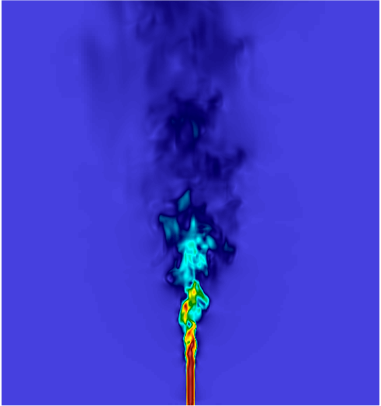
\includegraphics[width=0.65\textwidth]{figures/sco2_jet.png}
				\caption{Supercritical $CO_2$ jet}
			\end{figure}
			\begin{figure}
			    \centering
			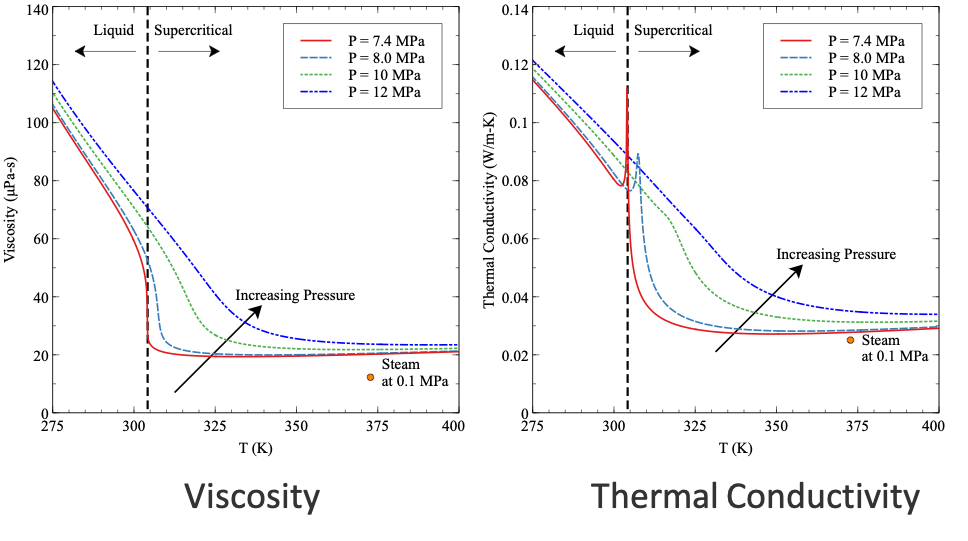
\includegraphics[width=0.82\textwidth]{figures/sco2nu.png}
			\caption{Variation in properties with $T$ for $CO_2$}
	\end{figure}



\subsection{Neural Net Architectures}

\begin{figure}
    \centering
    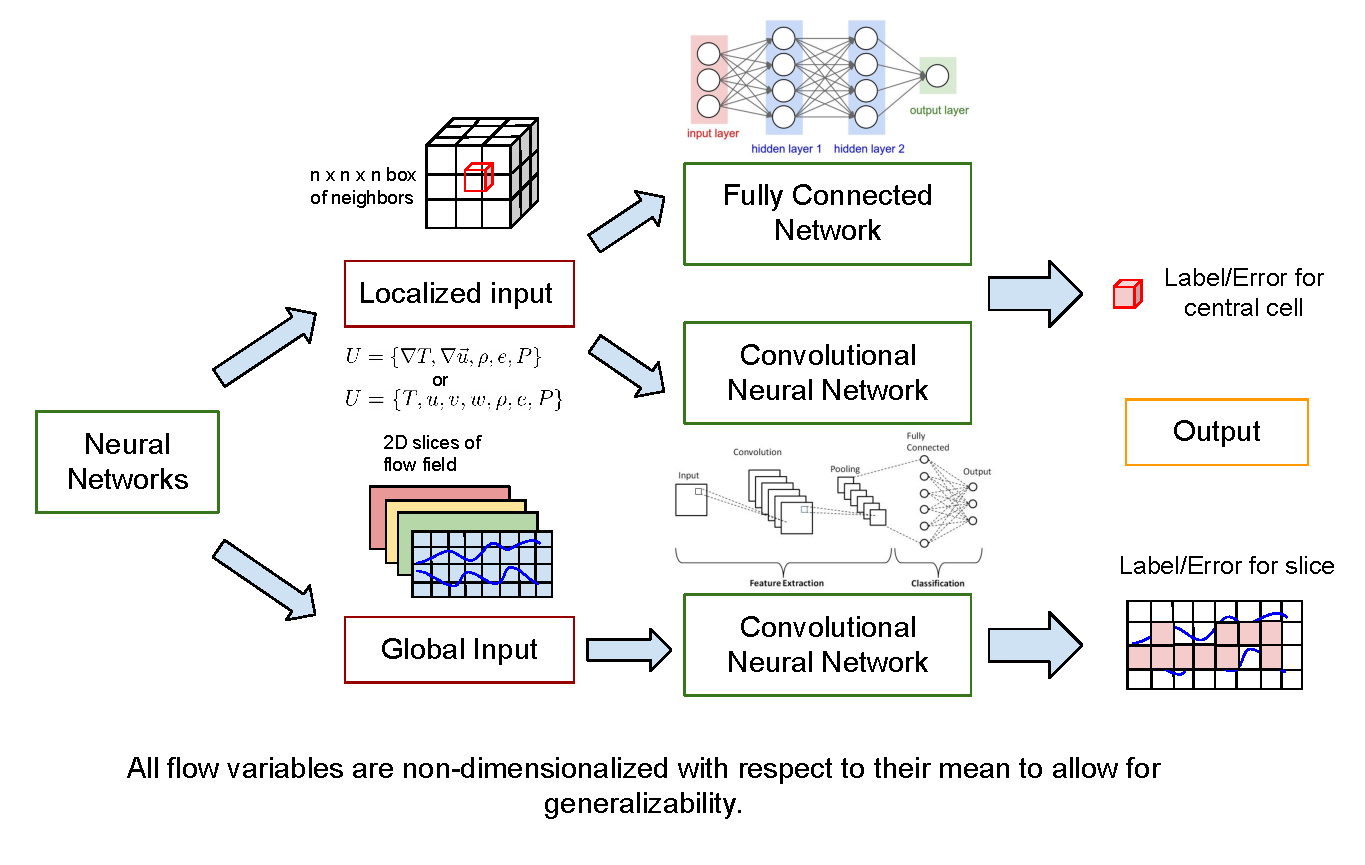
\includegraphics[width=\textwidth]{figures/NNs.pdf}
    \caption{Summary of architectures tested}
\end{figure}

The approaches can be broadly split into the following 2 categories:

\begin{enumerate}
    \item Localized input
    \begin{itemize}
        \item The state vector $x$ is provided in $n \times n \times n$ box as input to the neural net
        \item Raw input, $x = (T, \vec{u}, \rho, e, P)$ or grad input, $x = (\nabla T, \nabla \vec{u}, \rho, e, P)$
        \item Outputs label/error prediction for the central cell.
        \item Almost every grid cell is a training data point; points close to boundary removed for $n>1$ to ensure an $n \times n \times n$ box exists around the cell.
        \item Uses Malik's data downsampling algorithm to obtain a reasonable number of samples that uniformly samples the configuration state space.  
        \item Tested with a Fully connected network (FCNN) and Convolutional Neural Network (CNN) 
        \begin{itemize}
            \item FCNN ('regression.py'): Consists of 2 hidden layers; each hidden layer is followed by a batch normalization layer. There is a dropout layer before the final dense layer. 
            \item CNN ('regression\_cnn.py'): Consists of a 3D convolutional layer with kernel size $(3,3,3)$ with 4 filters followed by an Average Pooling layer with pool size = $(2,2,2)$. The output from the pooling layer is then flattened and fed to a dense layer. This is followed by dropout layer and the final output layer. Note: CNN requires $n \ge 5$
        \end{itemize}
    \end{itemize}
     All results in this document were generated using the grad input
    \item Global input
    \begin{itemize}
        \item The state vector $x$ is provided in $N_x \times N_y$ slice as input to the neural net
        \item Number of points z-indices is the number of training data available and is therefore limited given a single snapshot
        \item Output is the labeled slice or the predicted error on the slice.
        \item Tested with CNN ('regression\_cnn\_slices.py'): Input $\rightarrow$ Conv2D (filters = 32, kernel size = $(3,3)$) $\rightarrow$ Batch Normalization $\rightarrow$ Max Pooling (pool size = (2,2)) $\rightarrow$ Conv2D (filters = 16, kernel size = $(3,3)$) $\rightarrow$ Batch Normalization $\rightarrow$ Max Pooling (pool size = (2,2)) $\rightarrow$ Flatten $\rightarrow$ Dense(32) $\rightarrow$ Droput (0.11) $\rightarrow$ Dense(4) $\rightarrow$ Output)
    \end{itemize}
\end{enumerate}

Hyper paramater tuning was carried using sherpa. The results are summarized in Tables 1 and 2.  ReLu activation (except for sigmoid in final layer of classification) is used along with $L_1$ regularization. Mean squared error is chosen as the loss function in al cases.

\begin{table}
\centering
\begin{tabular}{llll}
 &Parameter  &Range   &Optimal    \\
 &Learning rate  &$[0.0001,0.001]$  &$0.0004$  \\
 &Dropout rate   &$[0,0.4]$  &$0.36$  \\
 &Batch size &${16,32,64,128,256}$  &128  \\
 &Hidden units (layer 1) & ${8,16,32,64,128}$  &64 \\
 &Hidden units (layer 2 & ${8,16,32,64,128}$  &128 \\
\end{tabular}
 \caption{Hyper parameter tuning for localized FCNN}
\end{table}

\begin{table}
\centering
\begin{tabular}{llll}
 &Parameter  &Range   &Optimal    \\
 &Learning rate  &$[0.0001,0.001]$  &$0.00013$  \\
 &Dropout rate   &$[0,0.4]$  &$0.11$  \\
 &Batch size &${16,32,64, 128,256}$  &32  \\
 &Number of filters & ${4,8,16,32,64}$  &4 \\
 &Hidden units & ${4,8,16,32}$  &8 \\
\end{tabular}
\caption{Hyper parameter tuning for localized CNN}
\end{table}

\subsection{Data preparation}
Data prep is mostly carried out inside the function:
\begin{verbatim}
    extract_from_pltfile()
\end{verbatim}

Main steps are:
\begin{enumerate}
    \item For state vector $x = (\nabla T, \nabla \vec{u}, \rho, e, P)$, the gradients are computed based on raw values; flow variables $\rho,\, e,\, P$ are non-dimensionalized with respect to their respective mean.
    \item Discretization error is computed by taking the difference between the non-dimensionalized $u$ (or $T$) from the filtered fine and coarse runs.
    \item Indices corresponding to the downsampled data are extracted for training.
    \item For FCNN, the $n \times n \times n \times n$ box is flattened after it is assembled. 
    \item The features are normalized using mean and standard deviation of training data. Label normalization is not necessary.
\end{enumerate}


\section{Results}

\subsection{A priori testing}

\subsubsection{Classification}

 \begin{figure}
    \centering
    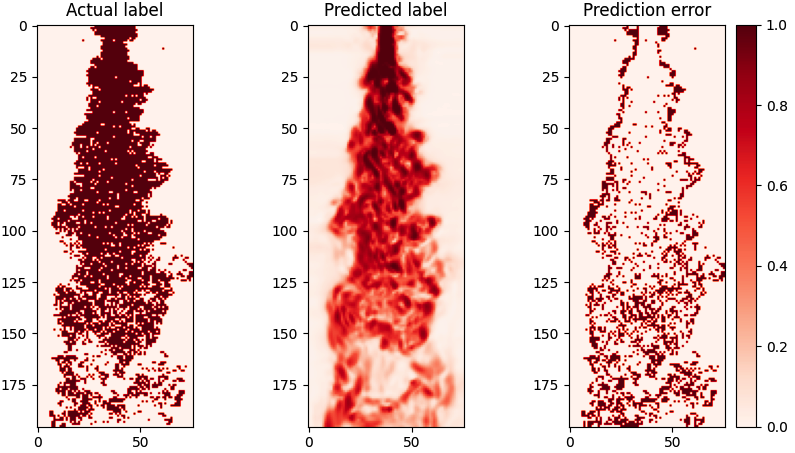
\includegraphics[width=0.8\textwidth]{figures/314_label.png}
    \caption{$T_{jet} = 314 K$, CNN (n=5, $\epsilon = 0.01$)}
\end{figure}
\begin{figure}
	\centering
	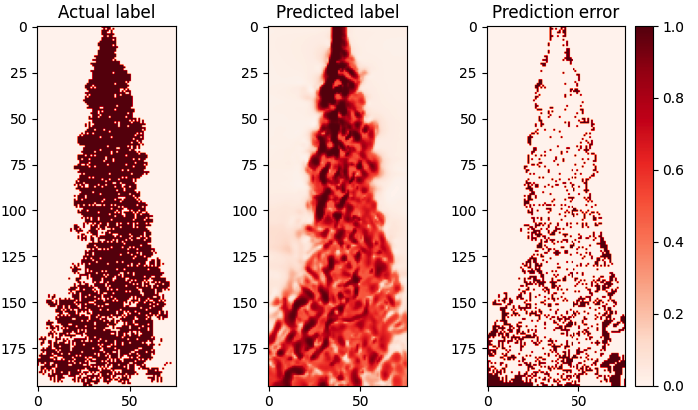
\includegraphics[width=0.8\textwidth]{figures/350_label.png}
	\caption{$T_{jet} = 350 K$, CNN (n=5, $\epsilon = 0.01$)}
\end{figure}

Key observations:
	\begin{itemize}
		\item All architectures perform reasonably well in the classification approach
		\item Neural nets are trained on a jet flow snapshot  ($T_{jet}=314 K, \epsilon = 0.01/0.1$) 
		\item ROC curve for $T_{jet}=350$ is shown in figure \ref{fig:roc}.
		\end{itemize}
		\begin{figure}
		    \centering
		    \includegraphics[width=0.7\textwidth]{figures/roc.png}
		    \caption{ROC curve for classification approach using CNN, n=5 }
		    \label{fig:roc}
		\end{figure}
		
		
\subsubsection{Regression}
 Key observations:
	\begin{itemize}
          \item Only localized CNN with $n\ge 5$ performs satisfactorily in the regression problem.
       	  \item Trained on a jet flow snapshot  ($T_{jet}=314 K$)
       	  \item FCNN (MSE $> 0.5$, $n=3$)and CNN slices (MSE $> 0.1$) fails to predict error accurately 
    \end{itemize}

\begin{figure}
    \centering
    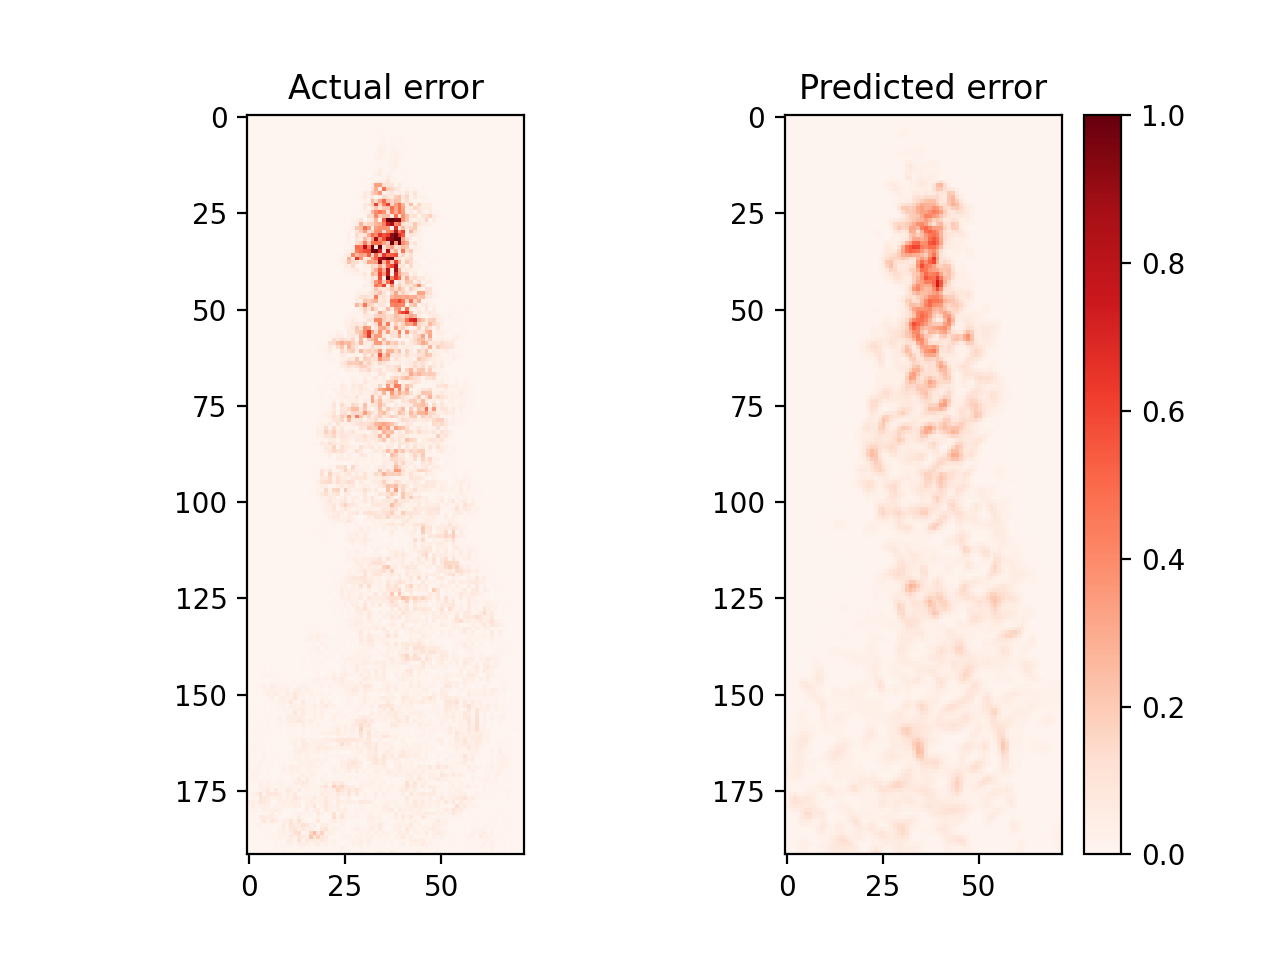
\includegraphics[width=0.8\textwidth]{figures/error_prediction_350.png}
    \caption{$T_{jet} = 350K$, CNN (n=9) error in $u$}
\end{figure}
\begin{figure}
	\centering
	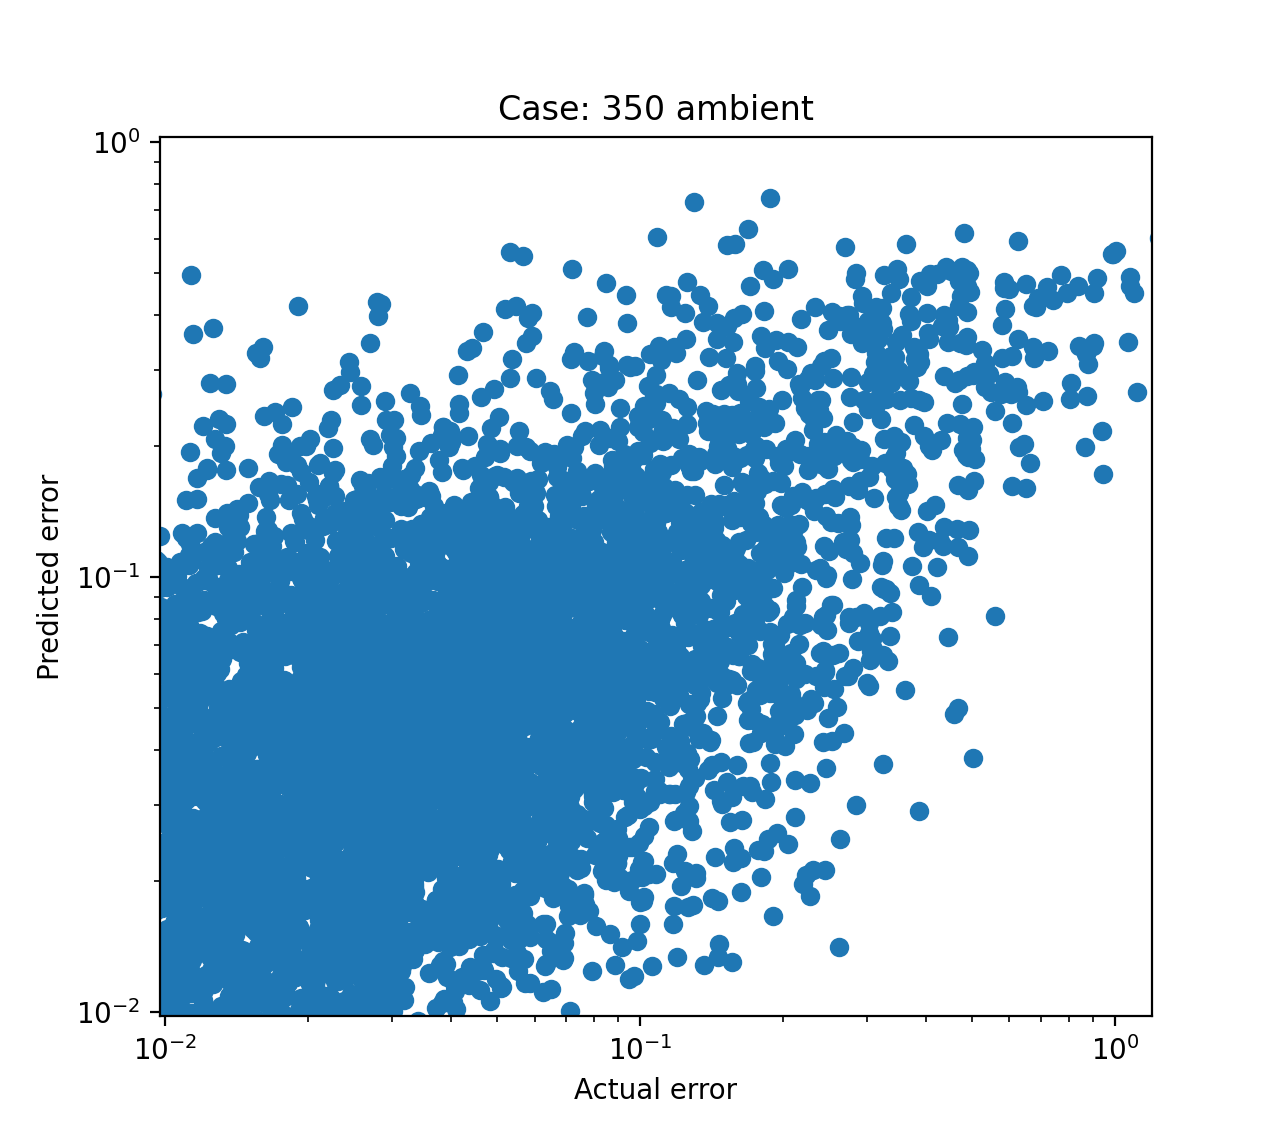
\includegraphics[width=0.65\textwidth]{figures/error_scatter_350.png}
	\caption{$T_{jet} = 350 K$, CNN (n=9) error in $u$}
\end{figure}

\begin{figure}
    \centering
    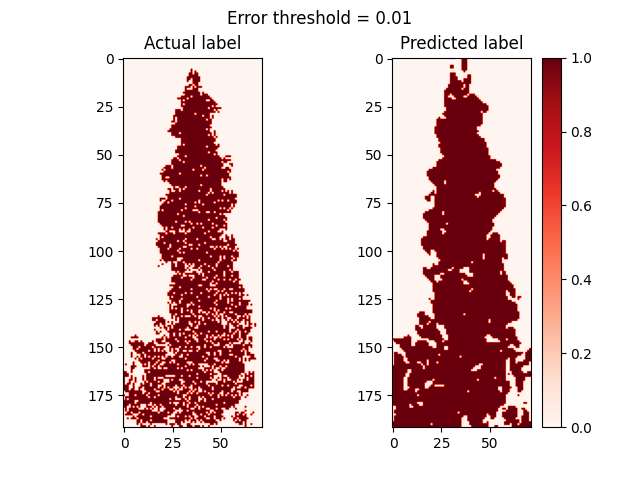
\includegraphics[width=0.7\textwidth]{figures/labeleps2.png}
    \caption{$T_{jet} = 350K$, CNN (n=9) labels based on error in $u$}
\end{figure}
\begin{figure}
	\centering
	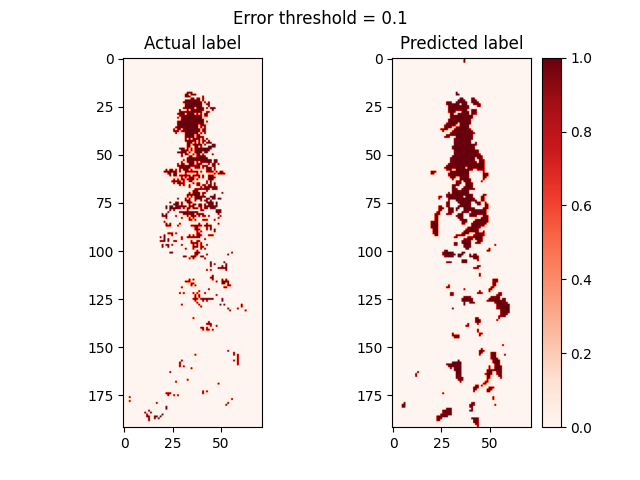
\includegraphics[width=0.7\textwidth]{figures/labeleps1.png}
	\caption{$T_{jet} = 350 K$, CNN (n=9) labels based on error in $u$}
\end{figure}

\subsection{Analysis of Neural Nets}

\subsubsection{Performance Comparison}

We carried out several tests to compare the performance of the various neural networks. 
\begin{enumerate}
    \item Performance with increase in number of neighbors for classification (Figure \ref{fig:nclass}) \\
    Observations:
    \begin{figure}
        \centering
        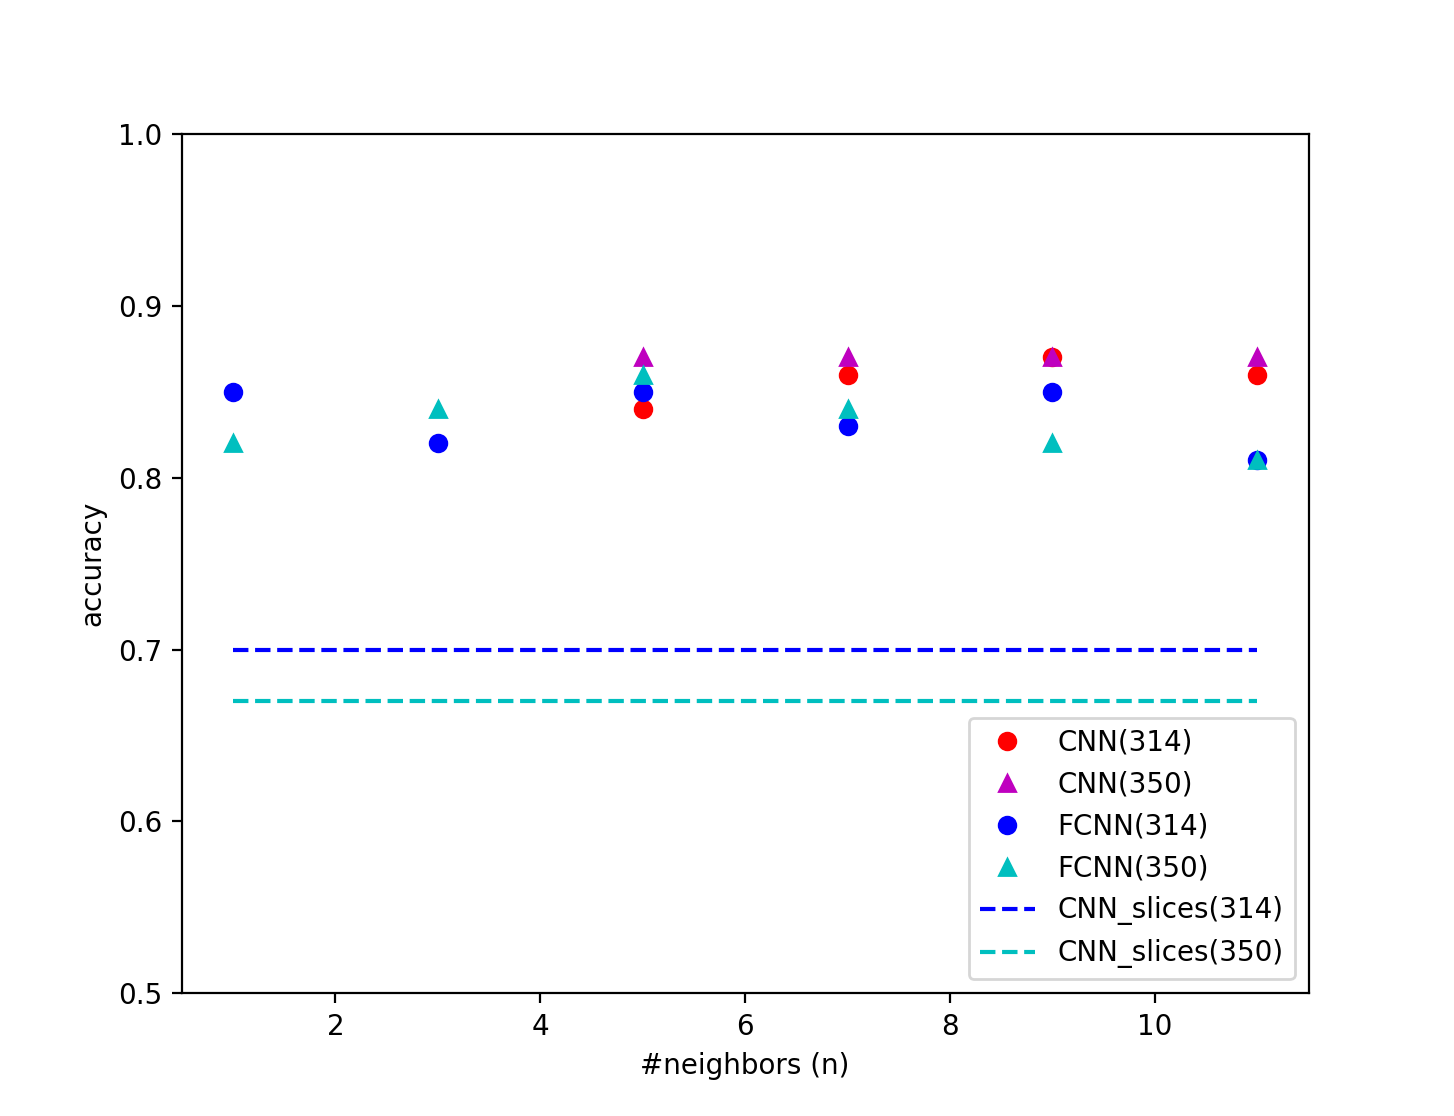
\includegraphics[width=0.7\textwidth]{figures/nclass.png}
        \caption{Variation in accuracy with increase in box size}
        \label{fig:nclass}
    \end{figure}
    \begin{itemize}
        \item Accuracy does not vary much with increase in box size
        \item This is consistent with the local nature of the dominant sources of error
        \item The local approach outperforms the global approach
    \end{itemize}
    \item Performance with increase in number of neighbors for regression (Figure \ref{fig:nreg}) \\
    \begin{figure}
        \centering
        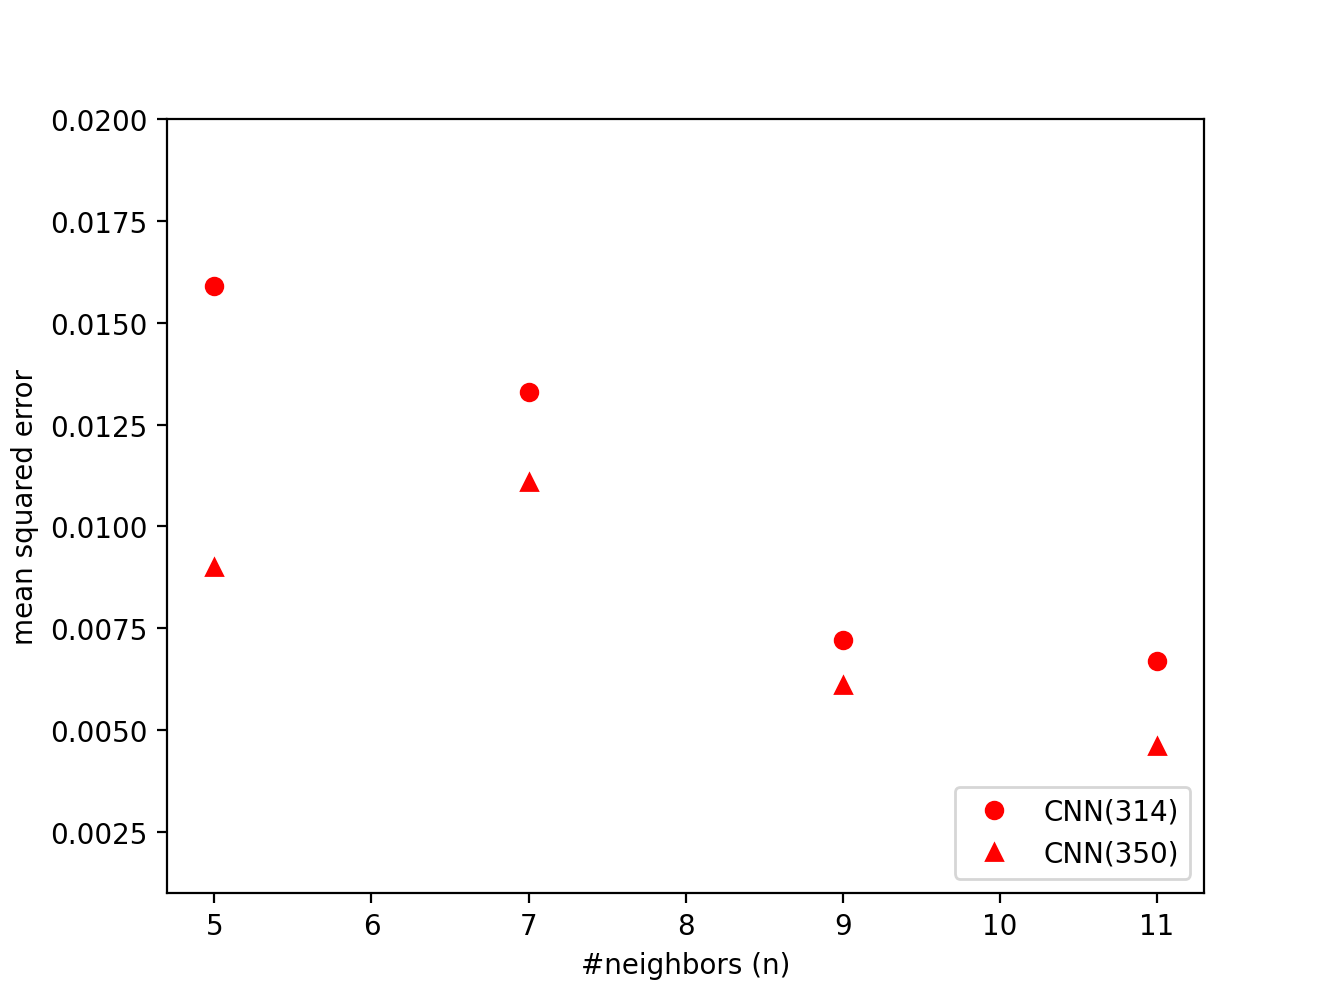
\includegraphics[width=0.7\textwidth]{figures/nreg.png}
        \caption{Variation in mean squared error with increase in box size}
        \label{fig:nreg}
    \end{figure}
    Observations:
    \begin{itemize}
        \item Mean squared error drops with increase in number of neighbors unlike in the classification problem
        \item This could be a result of the neural net computing higher order error terms using the neighbors
    \end{itemize}
    \item Performance variation with different state vectors, Grad ($\nabla T, \nabla u, \nabla v, \nabla w, \rho, e, P$) vs raw ($T, u, v, w, \rho, e, P$) for classification \\
    \begin{center}
        	\begin{tabular}{ |c|c|c|c| } 
    			\hline
    			n & Model(input) & Accuracy(314 K) & Accuracy(350 K)\\ 
    			\hline
    			1 & FCNN\color{red}{(raw)} & \color{red}0.83 & \color{red}0.65\\ 
    			1 &  FCNN(grad) & 0.85 & 0.82 \\ 
    			5 &  CNN\color{red}{(raw)} & \color{red}0.82 & \color{red}0.81 \\
    			5 &  CNN(grad) & 0.84 & 0.87 \\
    			\hline
    		\end{tabular} \\
    \end{center}
    Observations:
    \begin{itemize}
        \item Accuracy on the unseen $350 K$ case is higher using the grad input for both CNN (n=5) and FCNN (n=1)
        \item However, the performance of CNN on the unseen case is comparable using raw input to that of the grad input.
        \item This may be due to CNN computing gradients using the neighborhood info at some stage of the network; on the contrary, FCNN with a single input point is unable to compute gradients. 
    \end{itemize}
\end{enumerate}

\subsubsection{Feature Importance}

Permutation feature importance is used to study the relative importance of the input features for FCNN (n=1). Figure \label{fig:perm} shows the variation in mean squared error when the column corresponding to a particular feature is randomly permuted. We tried permuting pre-training and post-training. In the post-training approach, the features of the test data set are permuted after training. This is a good indicator of the dependence of the learned model on the different features (refer to lines 397 to 401 in regression.py). 

	\begin{figure}
	\centering
		\includegraphics[width=0.7\textwidth]{MSE.pdf}
		\caption{MSE variation on test set upon permuting inputs}
		\label{fig:perm}
	\end{figure}
	
		\begin{figure}
		\centering
    	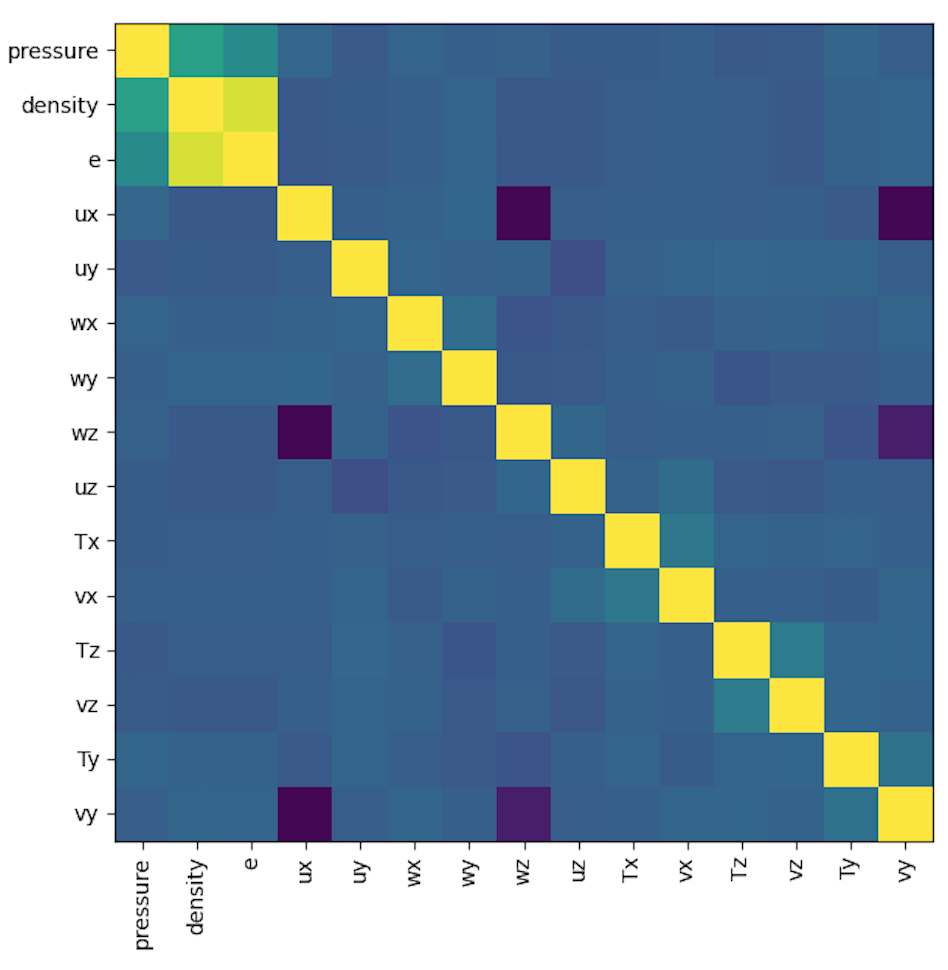
\includegraphics[width=0.6\textwidth]{figures/spearman_heatmap.png}
    	\caption{Spearman correlation: Indicates montonic relationship}
    \end{figure}

From figure \ref{fig:perm}, the trained model seems to rely heavily on $T_x$ and velocity gradients to make the predictions.The pre-training approach indicates that the mean squared error is most affected by permutation of velocity gradients. These results are commensurate with our understanding of error arising from subgrid scale stresses (refer to lines 197 to 200 in regression.py).

We also computed the Spearman correlation of the different features to identify variables that are monotonically related. The results indicate that Pressure, density and internal energy are highly correlated and therefore any two of them could be discarded without affecting model performance. However, the permutation feature importance results show that these variables have little to no bearing on the performance. Therefore, all three can be removed without affecting performance. This was verified by testing. 

\subsection{A posteriori testing}

The main steps of the implementation are as follows:

	\begin{itemize}
		\item ML Model is developed in Tensorflow.
		\item C API library is used to call the saved model from PeleC
		\item Tensorflow model is loaded in prob.cpp (amrex\_probinit)
		\item Input tensor is prepared inside set\_problem\_tags in prob.H and evaluated by model
		\item If predicted label is greater than 0.5, the cell is tagged for refinement
	\end{itemize}
	
\begin{figure}
        \centering
		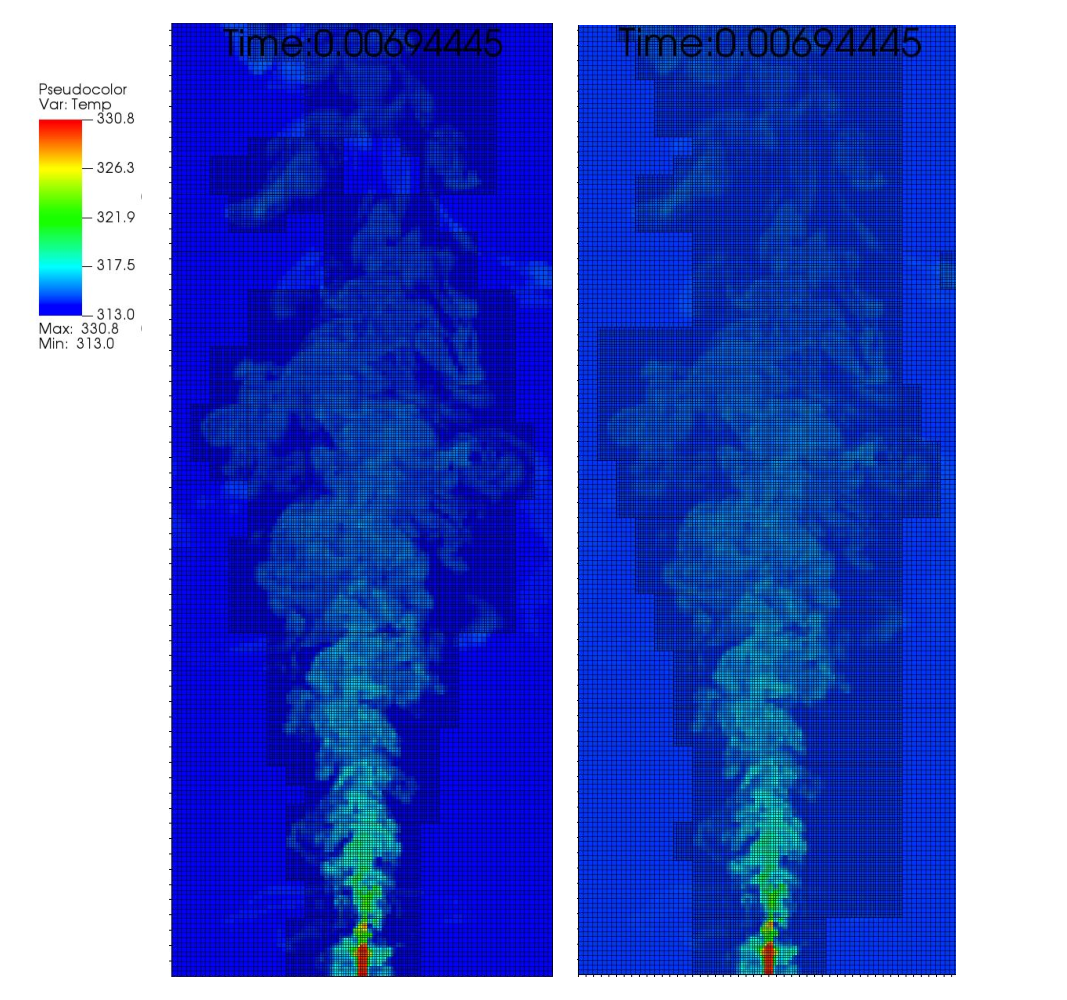
\includegraphics[width=0.8\textwidth]{figures/lvl1.pdf}
		\caption{ (Left) Existing tagging, (Right) FCNN (n=1) in PeleC}
\end{figure}
Key observations:
	\begin{itemize}
			\item Level 1 refinement for existing tagging: 33.1 \%
			\item Level 1 refinement for FCNN ($\epsilon = 0.01$): 35.6\%
			\item Tags close to $8\%$ of cells
		\end{itemize}

\section{Conclusions}

\begin{itemize}
		\item FCNN, CNN with local and global input (slices) are found to be successful in classifying cells based on an error threshold.
		\item Classifiation performance does not vary significantly with size of input $n$ - this is commensurate with the localized nature of spatial discretization error and subgrid scale stresses.
		\item Local CNN outperforms other approaches in error prediction
	\end{itemize}
	
\section{Future work}

 \begin{itemize}
 	\item Analysis for higher levels of refinement in PeleC
 	\item Feature importance study for regression to probe sources of error
 	\item ML-LES by extending regression (error prediction) approach 
 \end{itemize}

\newpage
\section{Old notes}

\begin{figure}
    \centering
    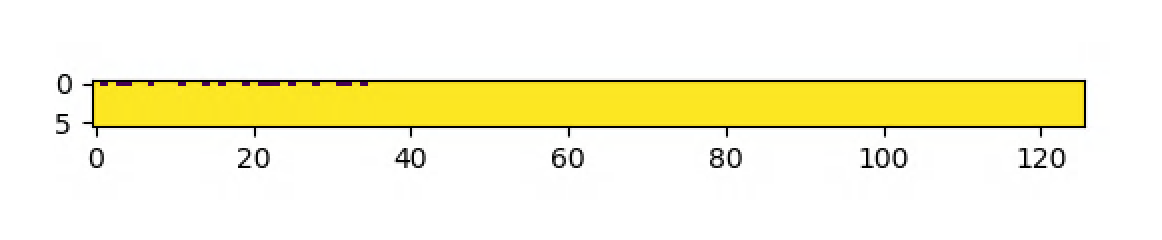
\includegraphics[width = 0.8\linewidth]{figures/ML_AMR_PMF.png}
    \caption{Plot showing areas in the domain prone to learning error.}
    \label{amr_err}
\end{figure}

\paragraph{314 ambient on base grid}

\begin{figure}[h!]
    \centering
    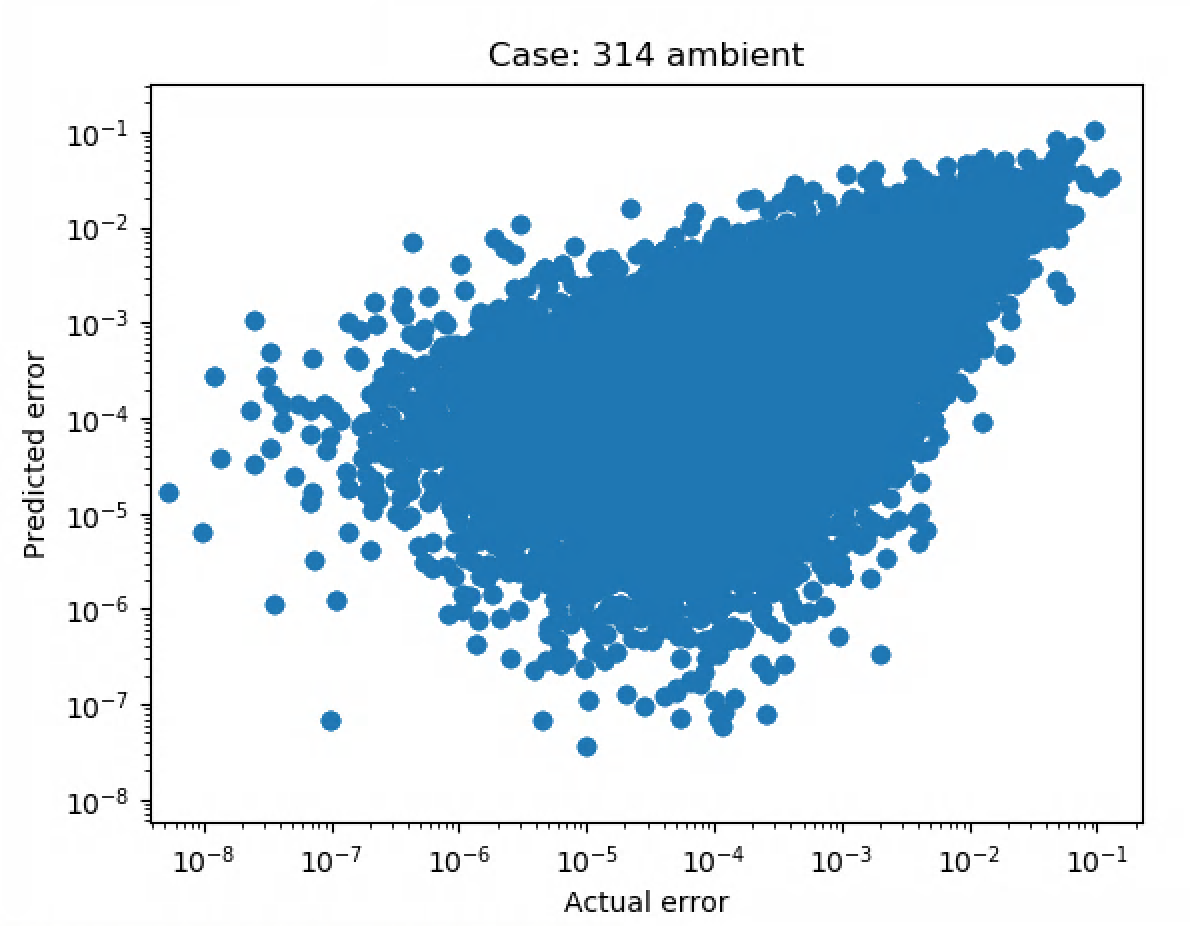
\includegraphics[width = 0.6\linewidth]{figures/314_01_error_scatter.png}
    \caption{Scatter plot showing actual vs predicted error (Case: 350 ambient jet)}
    \label{amr_err}
\end{figure}

\begin{figure}[h!]
    \centering
    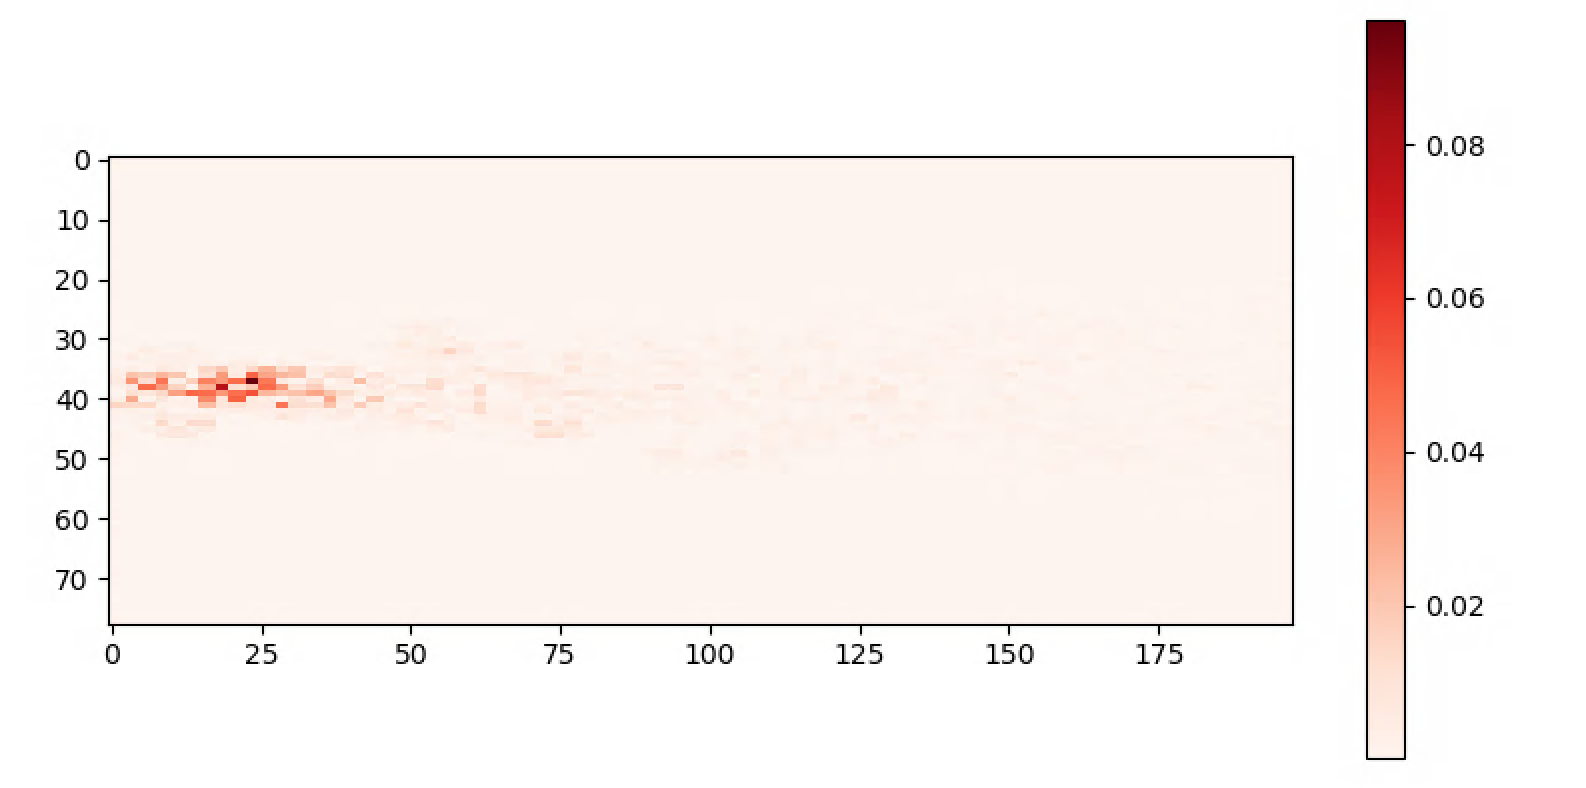
\includegraphics[width = 0.85\linewidth]{figures/314_01_actual.png}
    \caption{Plot showing actual error in $u$ computed from from level 1 run (Case: 314 ambient jet).}
    \label{amr_err}
\end{figure}

\begin{figure}[h!]
    \centering
    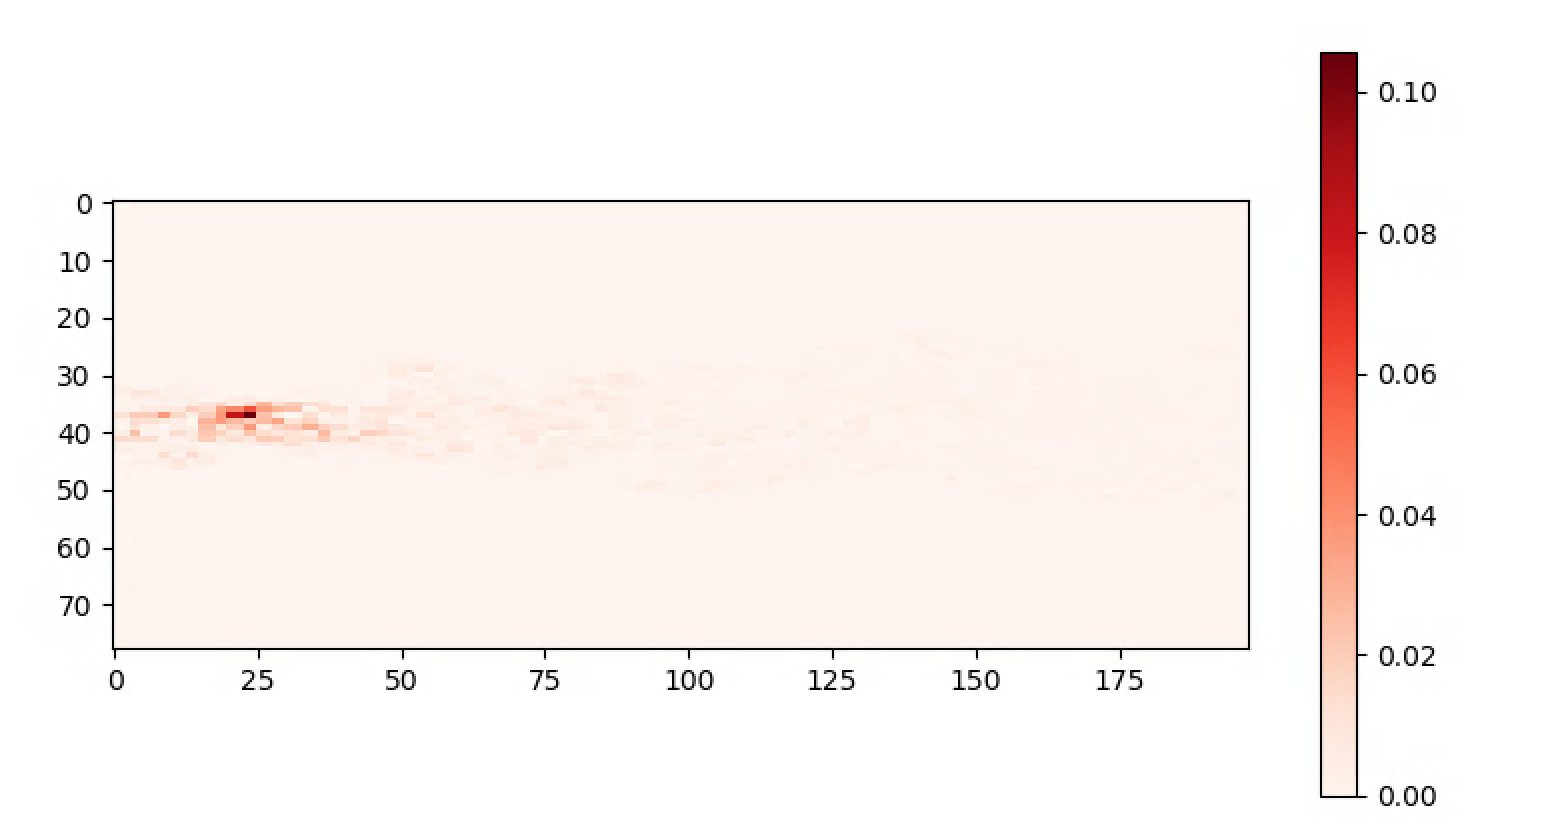
\includegraphics[width = 0.8\linewidth]{figures/314_01_pred.png}
    \caption{Plot showing predicted error in $u$.}
    \label{amr_err}
\end{figure}

\begin{figure}[h!]
    \centering
    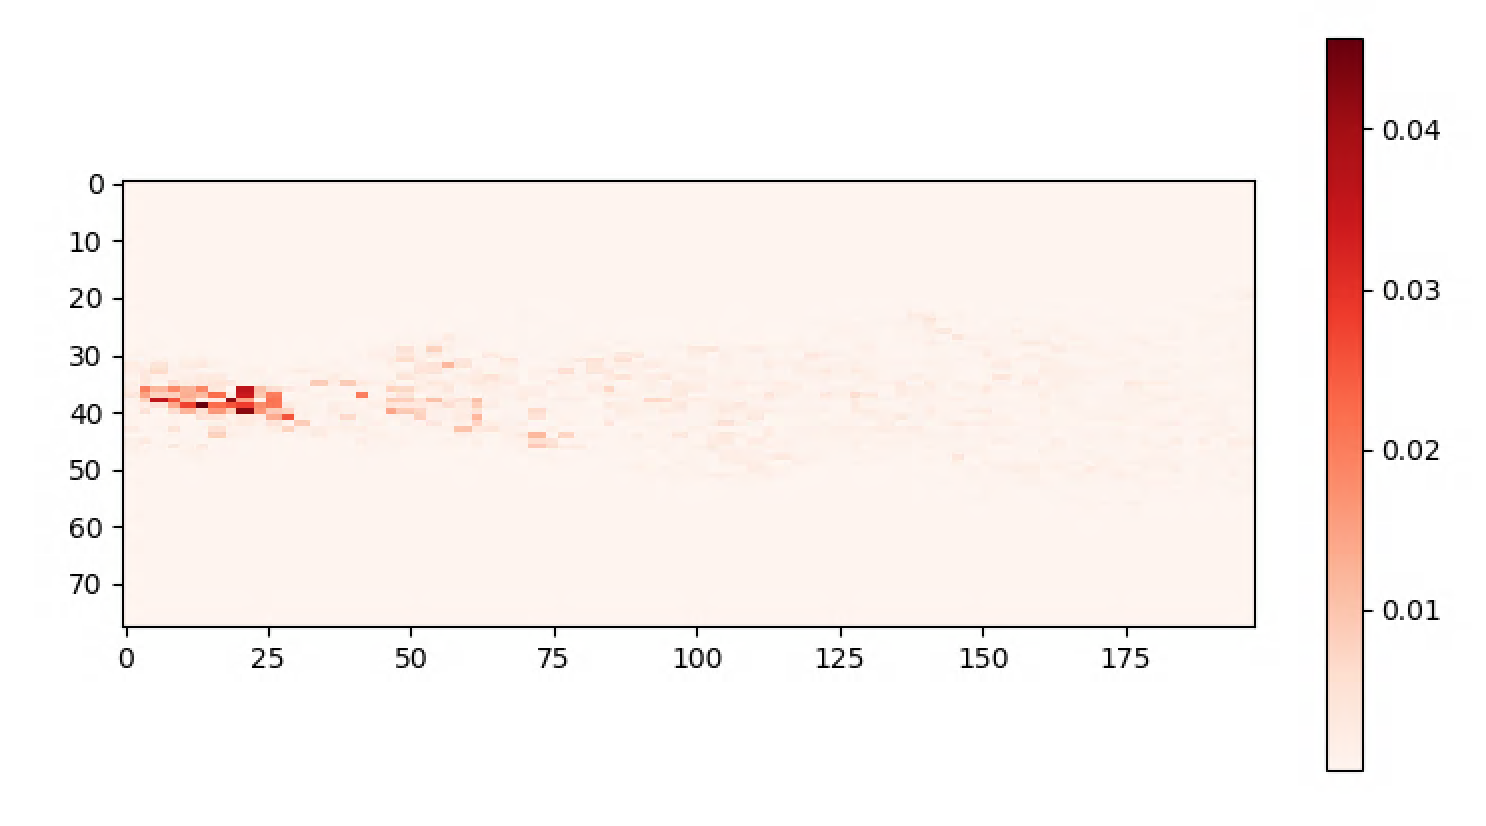
\includegraphics[width = 0.9\linewidth]{figures/314_01_error.png}
    \caption{Plot showing learning error (Case: 314 ambient jet)}
    \label{amr_err}
\end{figure}

\begin{figure}[h!]
    \centering
    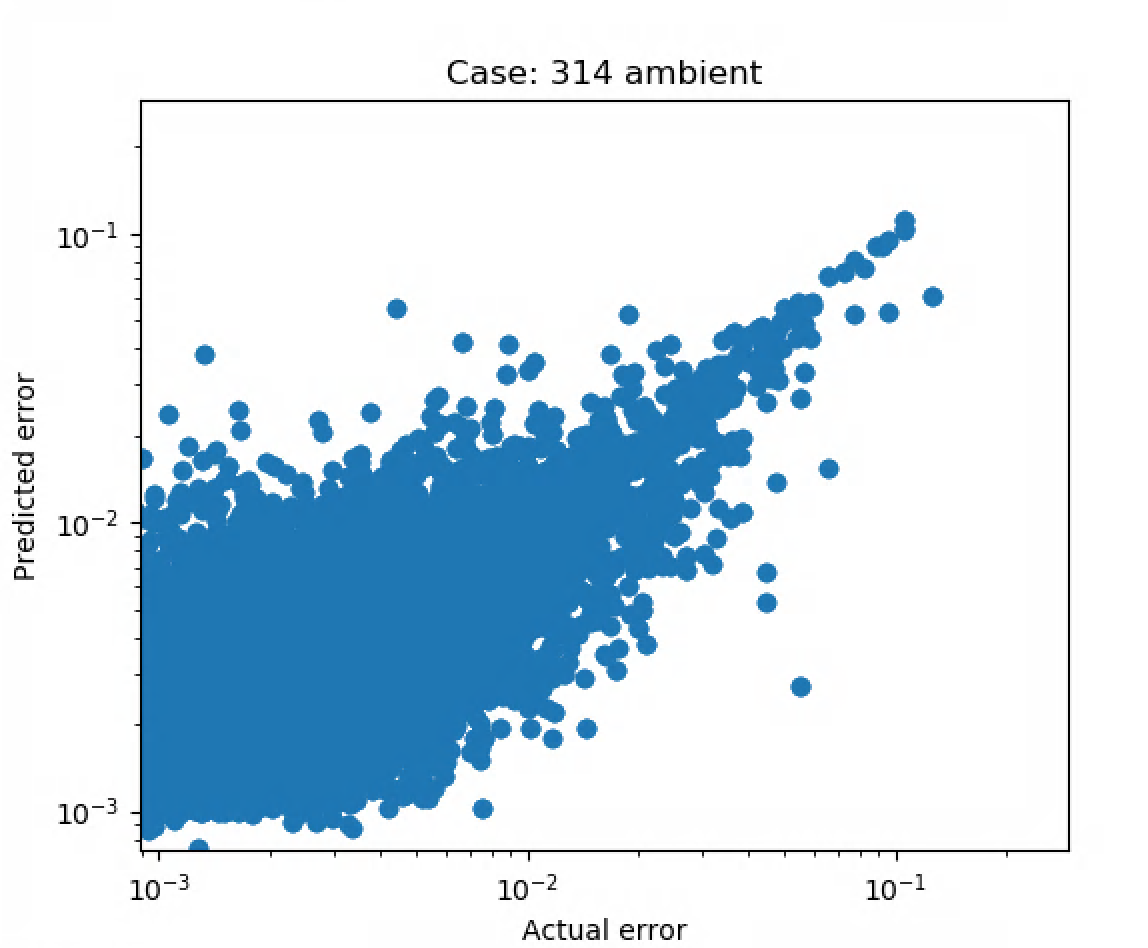
\includegraphics[width = 0.6\linewidth]{figures/314_01_grad_error_scatter.png}
    \caption{Scatter plot showing actual vs predicted error (Case: 350 ambient jet gradient)}
    \label{amr_err}
\end{figure}

\begin{figure}[h!]
    \centering
    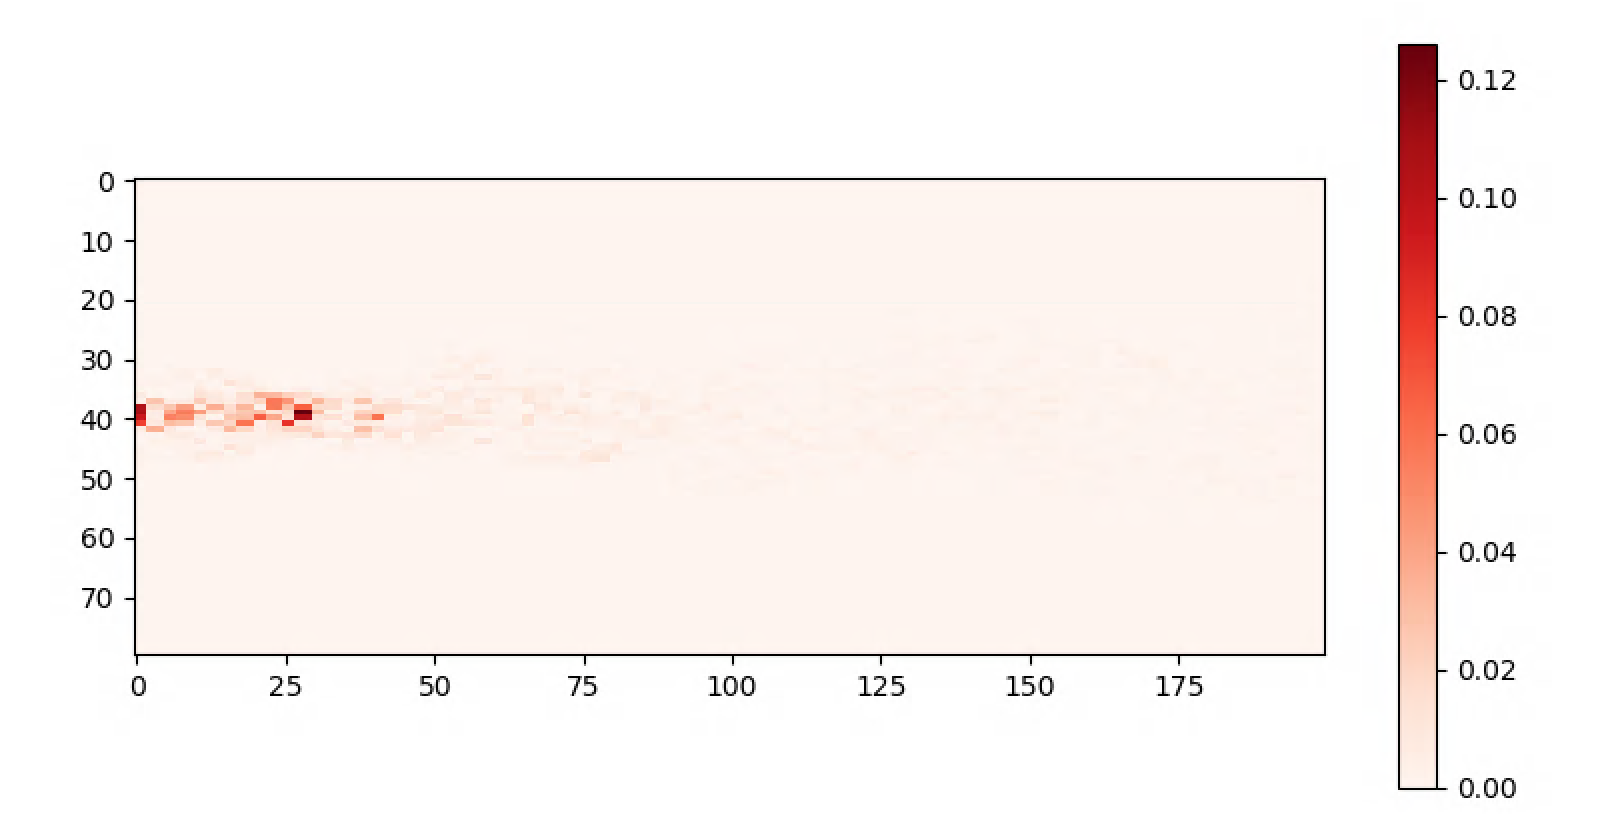
\includegraphics[width = 0.85\linewidth]{figures/314_01_grad_actual.png}
    \caption{Plot showing actual error in $T$ computed from from level 1 run (Case: 314 ambient jet gradients).}
    \label{amr_err}
\end{figure}

\begin{figure}[h!]
    \centering
    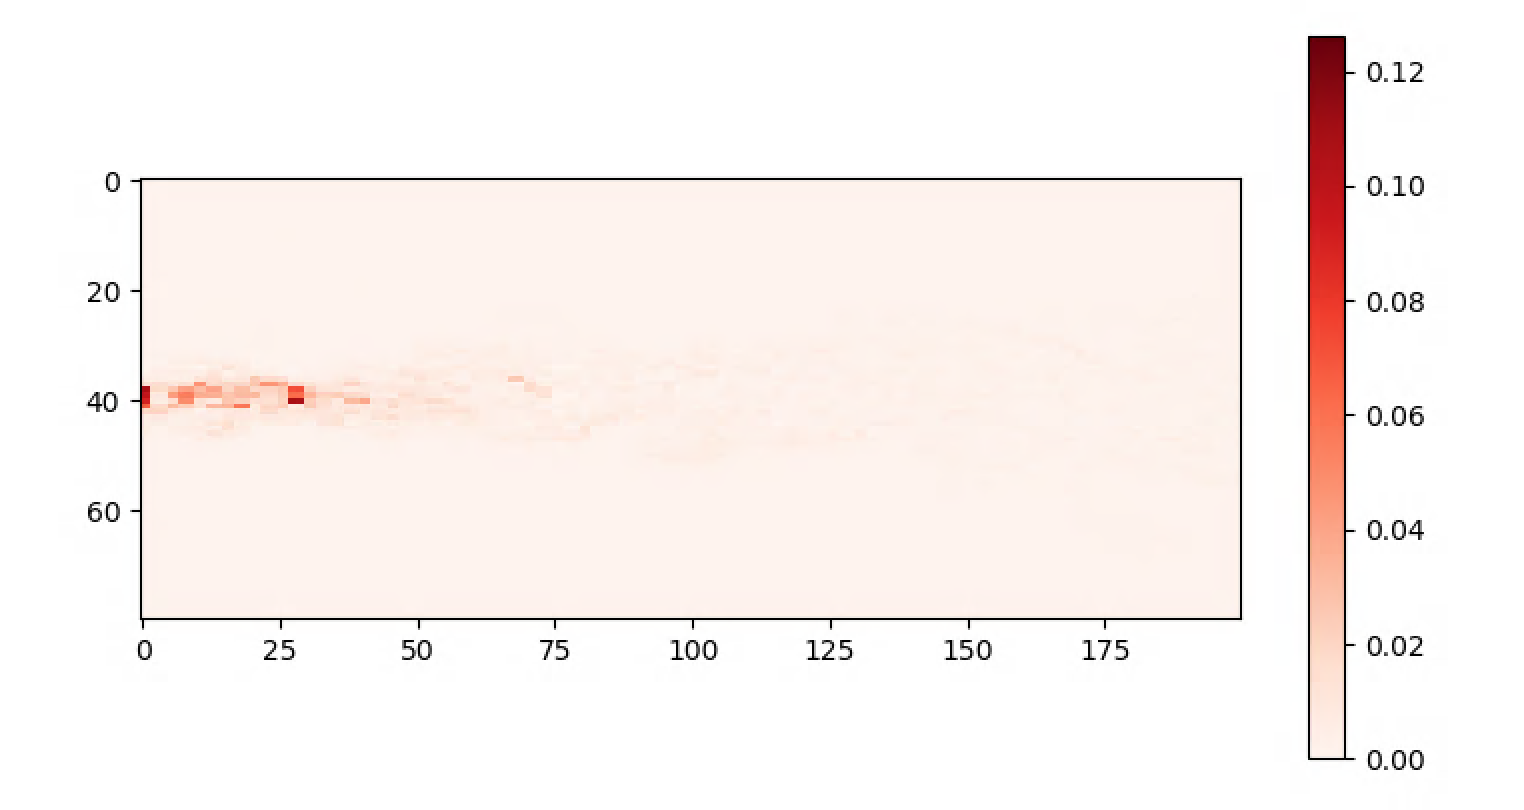
\includegraphics[width = 0.8\linewidth]{figures/314_01_grad_pred.png}
    \caption{Plot showing predicted error in $T$.}
    \label{amr_err}
\end{figure}

\begin{figure}[h!]
    \centering
    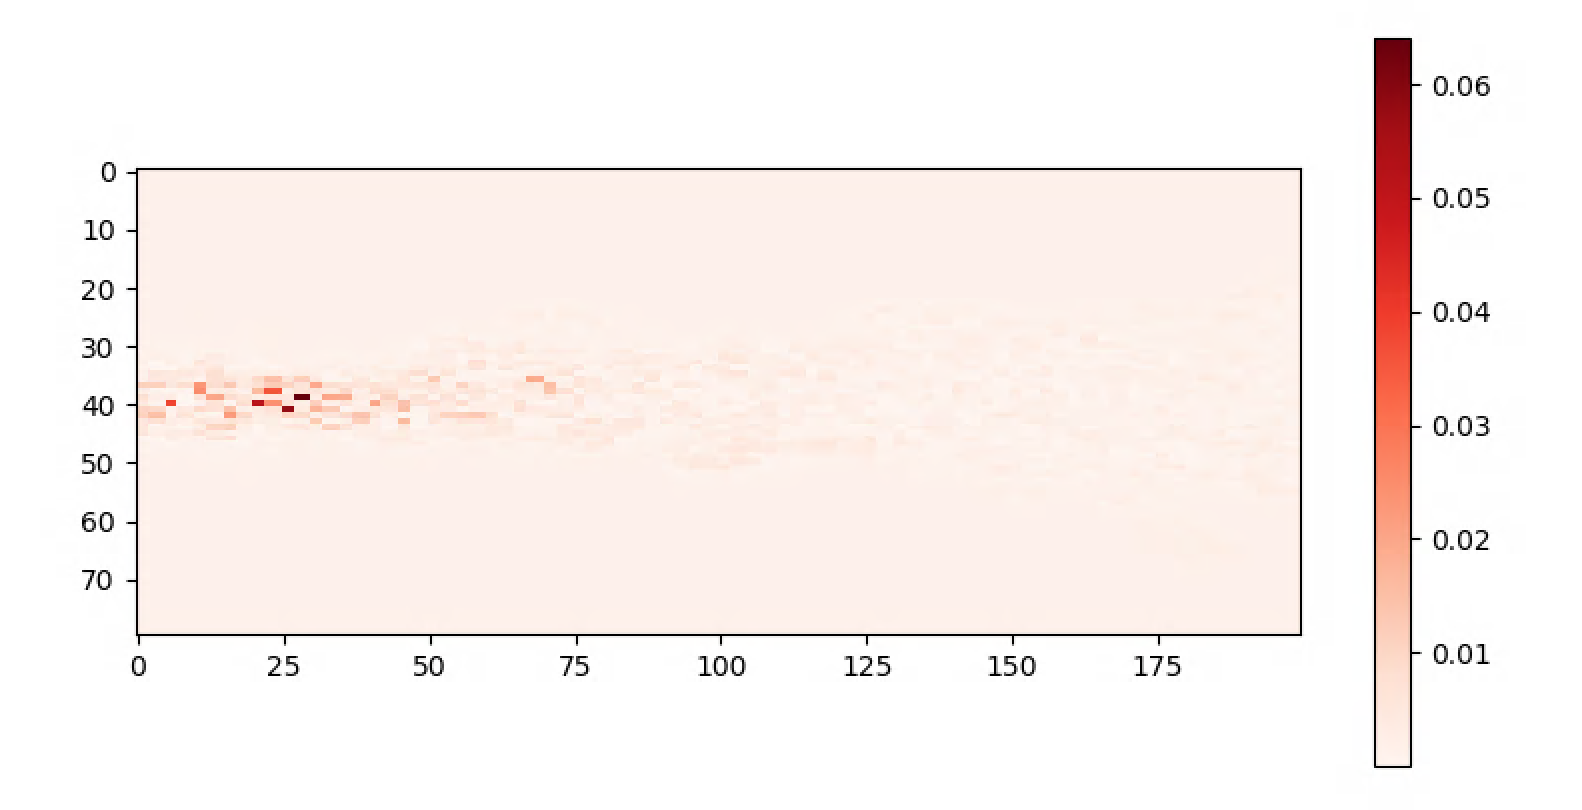
\includegraphics[width = 0.9\linewidth]{figures/314_01_grad_error.png}
    \caption{Plot showing learning error (Case: 314 ambient jet)}
    \label{amr_err}
\end{figure}

\paragraph{314 ambient on level 1 grid}

\paragraph{350 ambient on base grid}

\begin{figure}[h!]
    \centering
    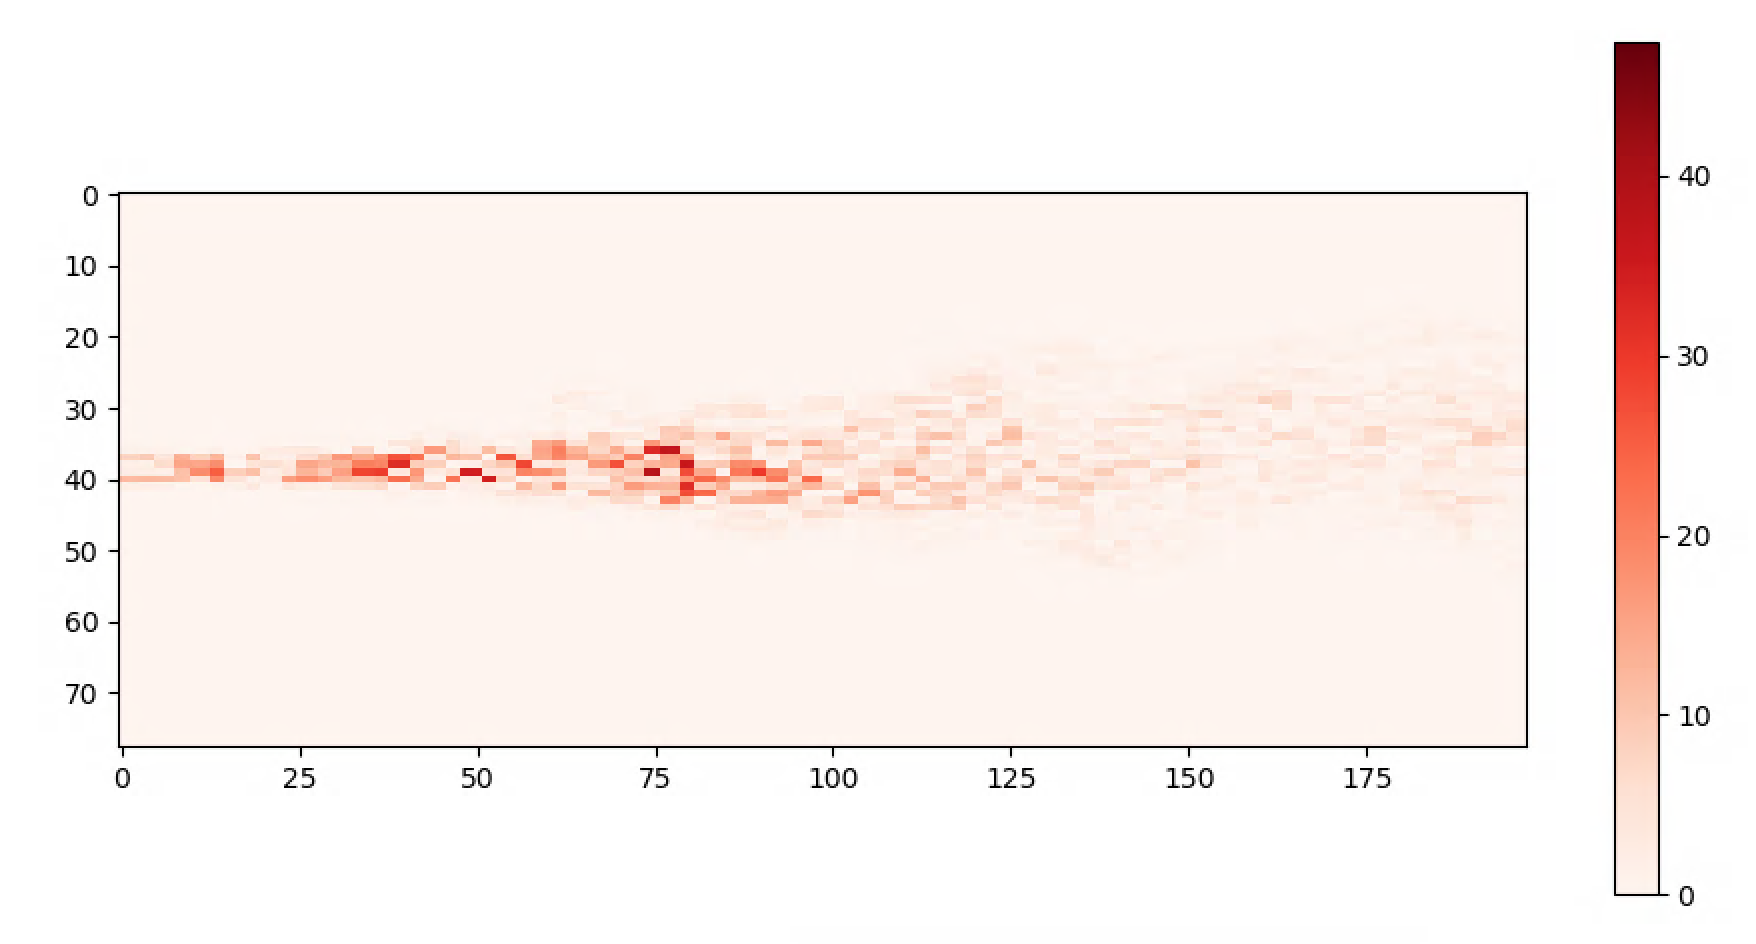
\includegraphics[width = 0.8\linewidth]{figures/350_01_actual.png}
    \caption{Plot showing actual error in $u$ computed from from level 1 run (Case: 350 ambient jet).}
    \label{amr_err}
\end{figure}

\begin{figure}[h!]
    \centering
    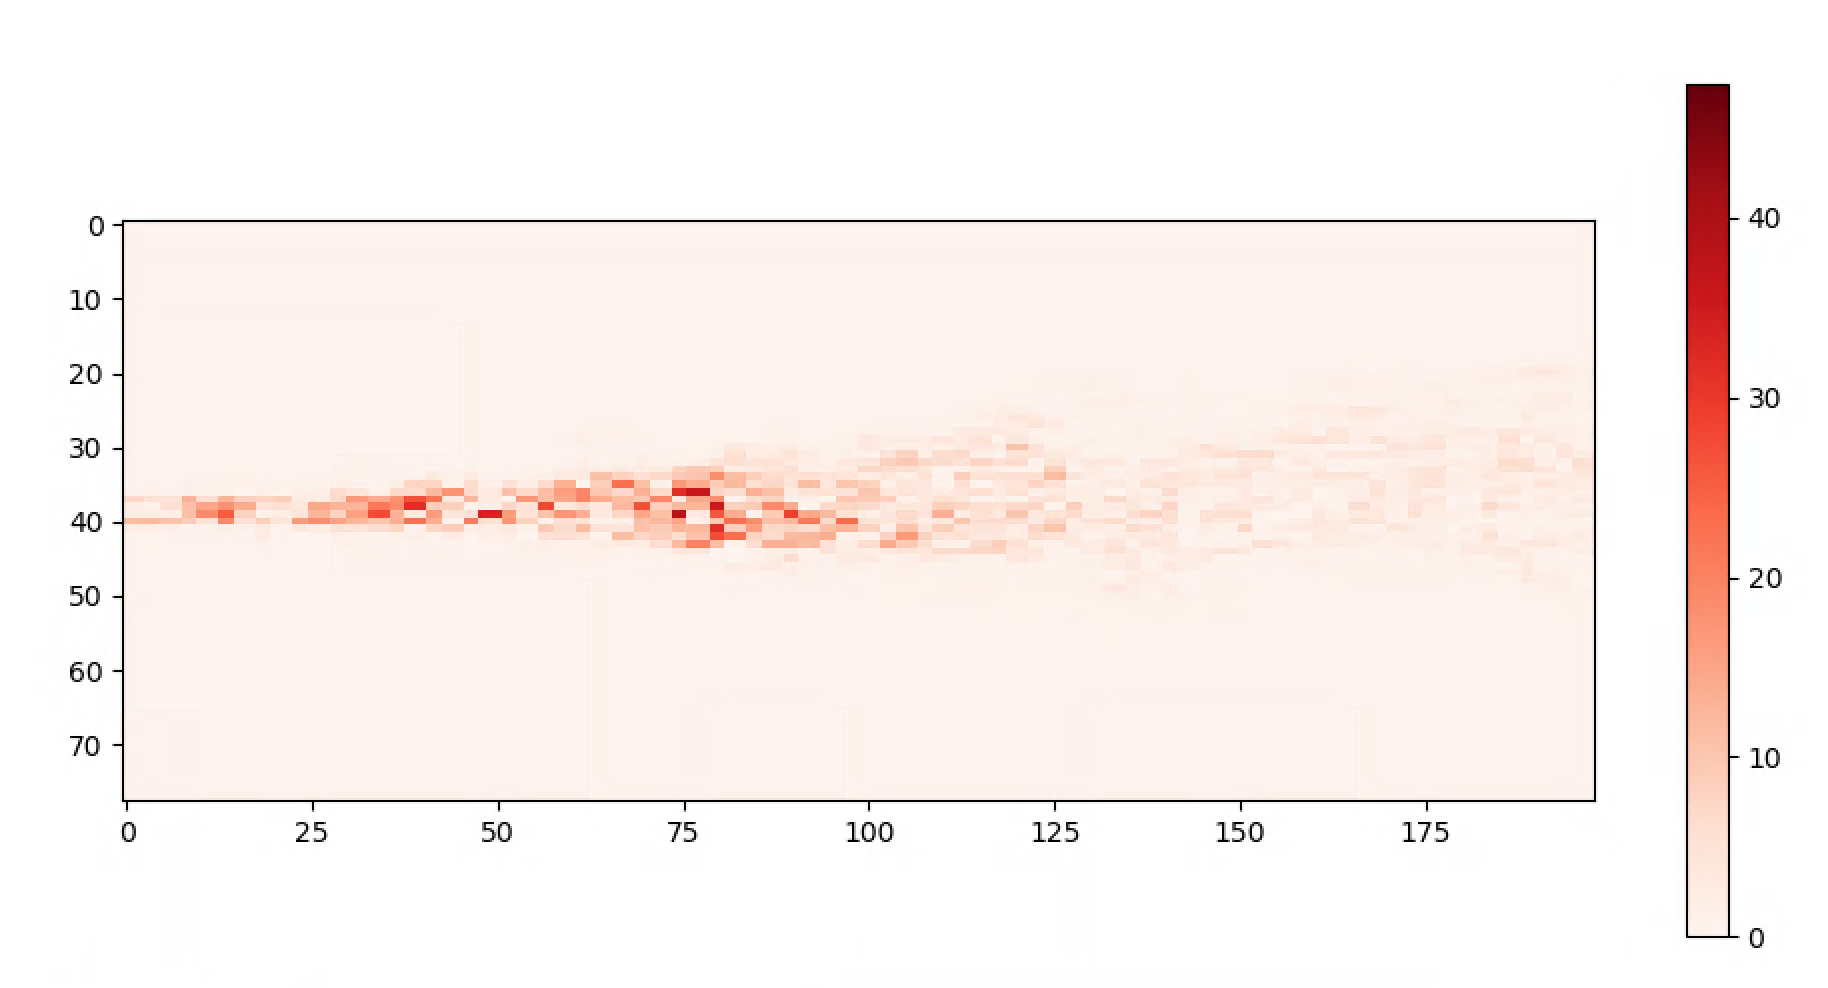
\includegraphics[width = 0.8\linewidth]{figures/350_01_pred.png}
    \caption{Plot showing predicted error in $u$ (Case: 350 ambient jet).}
    \label{amr_err}
\end{figure}

\begin{figure}
    \centering
    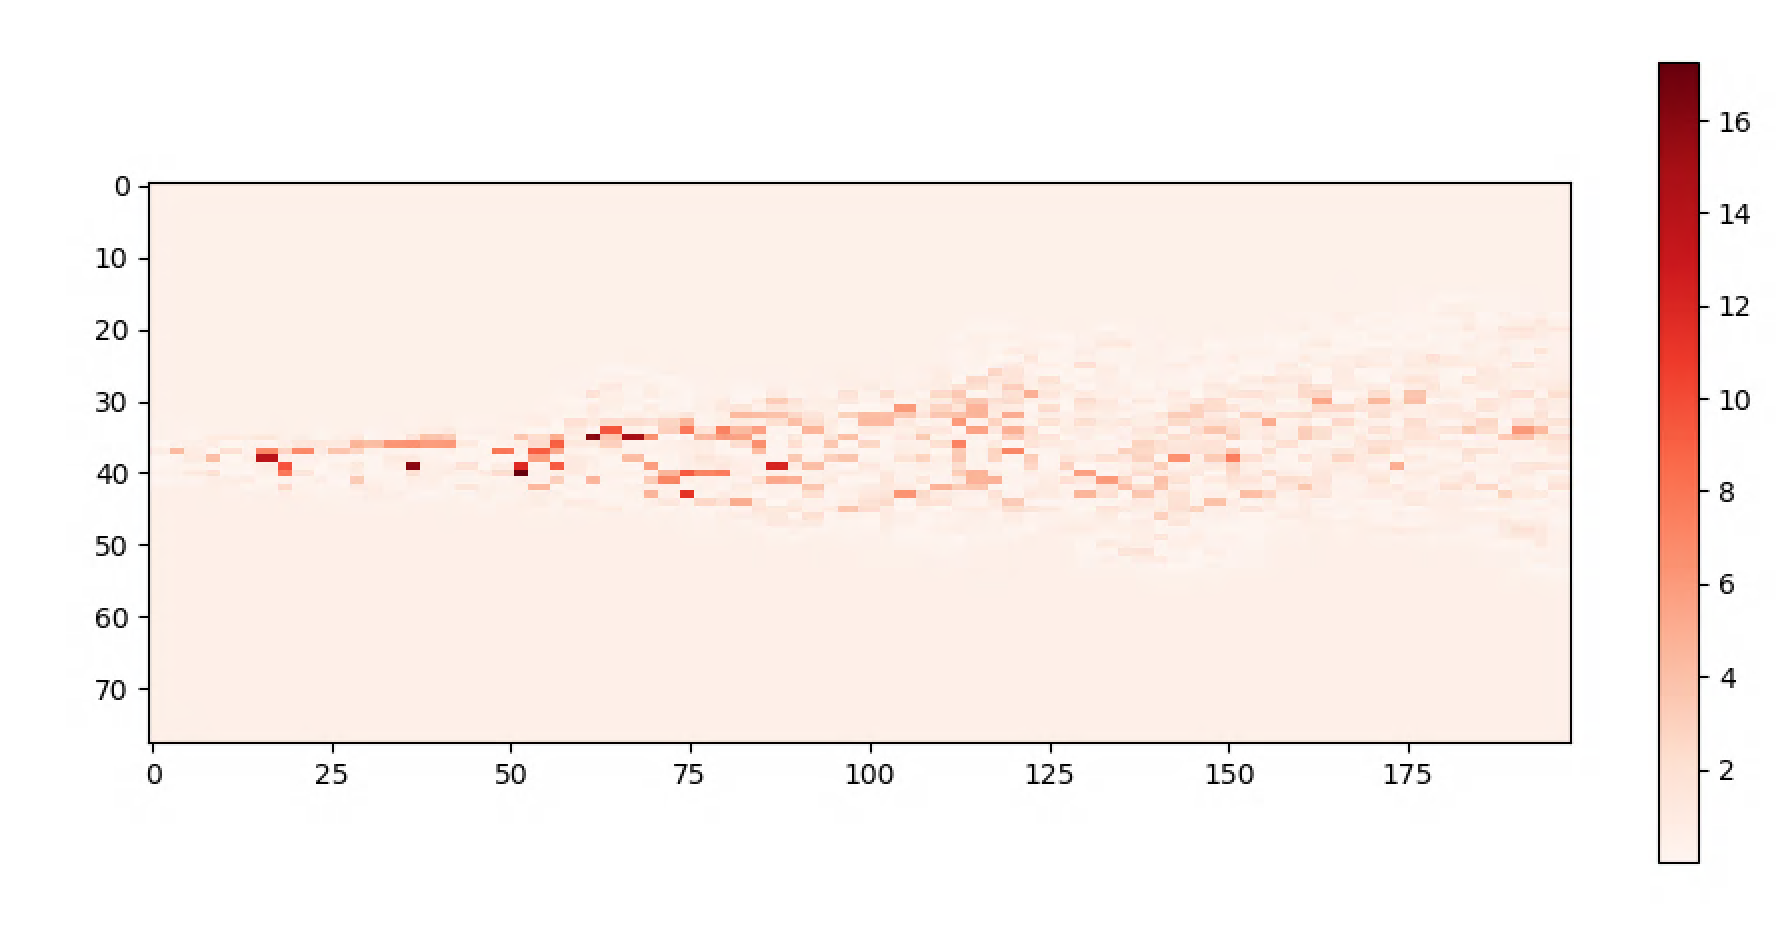
\includegraphics[width = 0.5\linewidth]{figures/350_01_error.png}
    \caption{Plot showing learning error (Case: 350 ambient jet)}
    \label{amr_err}
\end{figure}

\begin{figure}
    \centering
    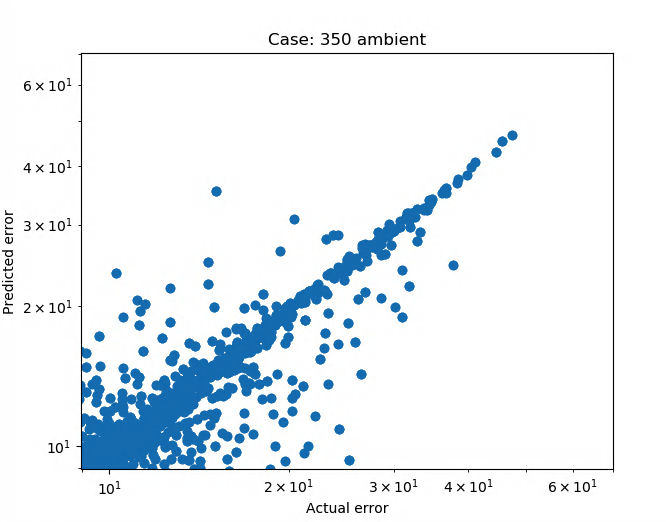
\includegraphics[width = 0.6\linewidth]{figures/error_scatter_350_01.png}
    \caption{Scatter plot showing actual vs predicted error (Case: 350 ambient jet)}
    \label{amr_err}
\end{figure}

\paragraph{350 ambient on level 1 grid}

\begin{figure}[h!]
    \centering
    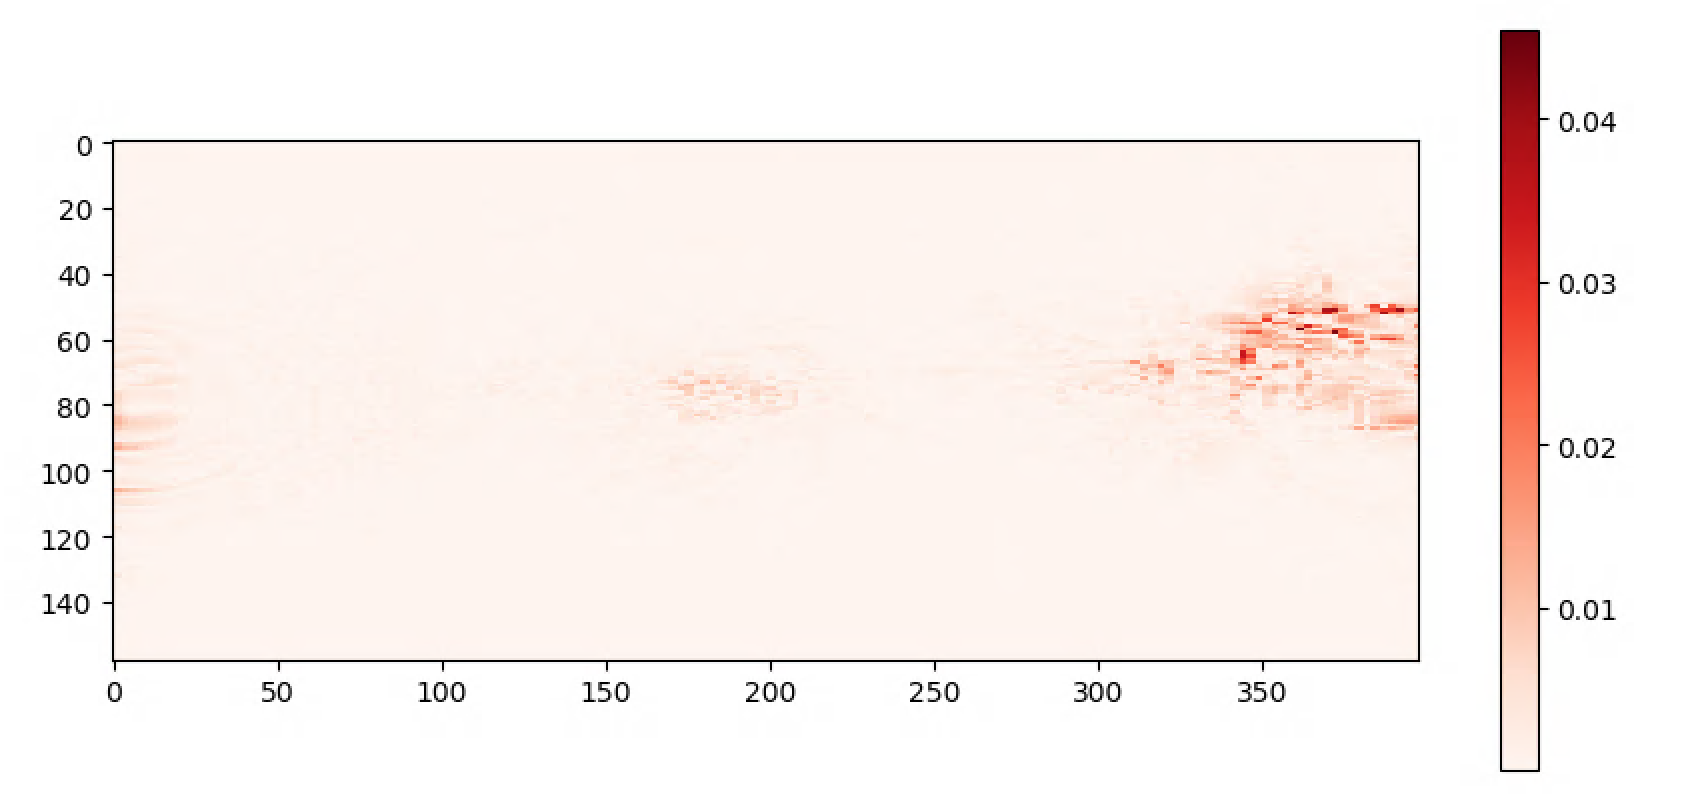
\includegraphics[width = 0.8\linewidth]{figures/350_12_actual.png}
    \caption{Plot showing actual error computed from from level 2 run (Case: 350 ambient jet).}
    \label{amr_err}
\end{figure}

\begin{figure}[h!]
    \centering
    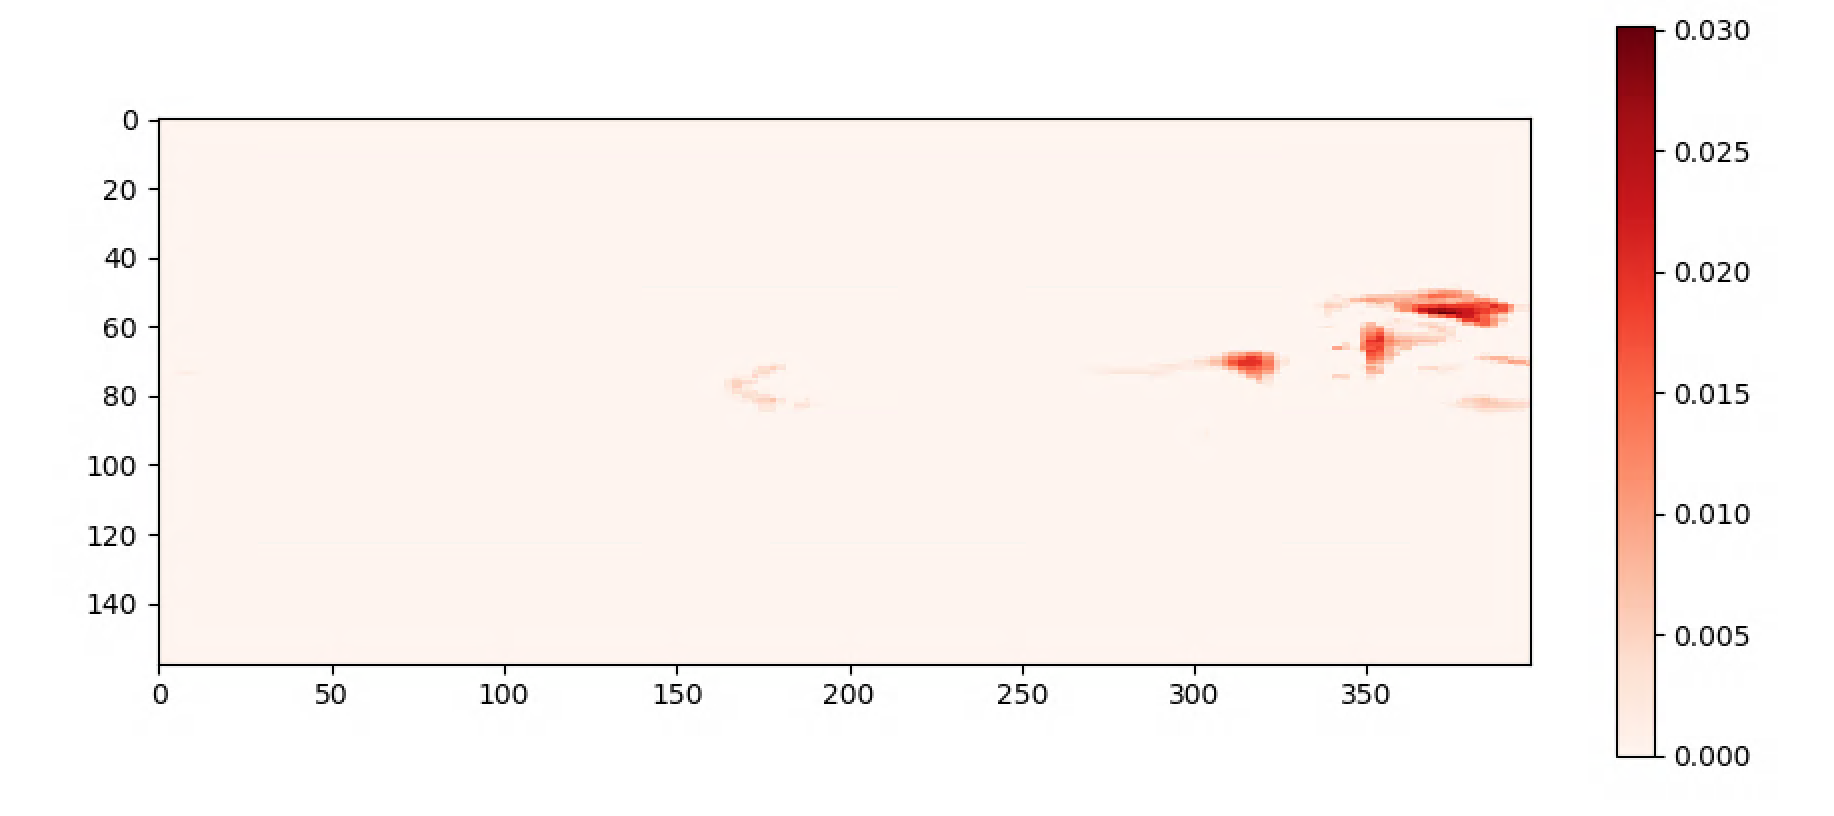
\includegraphics[width = 0.8\linewidth]{figures/350_12_pred.png}
    \caption{Plot showing predicted error (Case: 350 ambient jet).}
    \label{amr_err}
\end{figure}

\begin{figure}[h!]
    \centering
    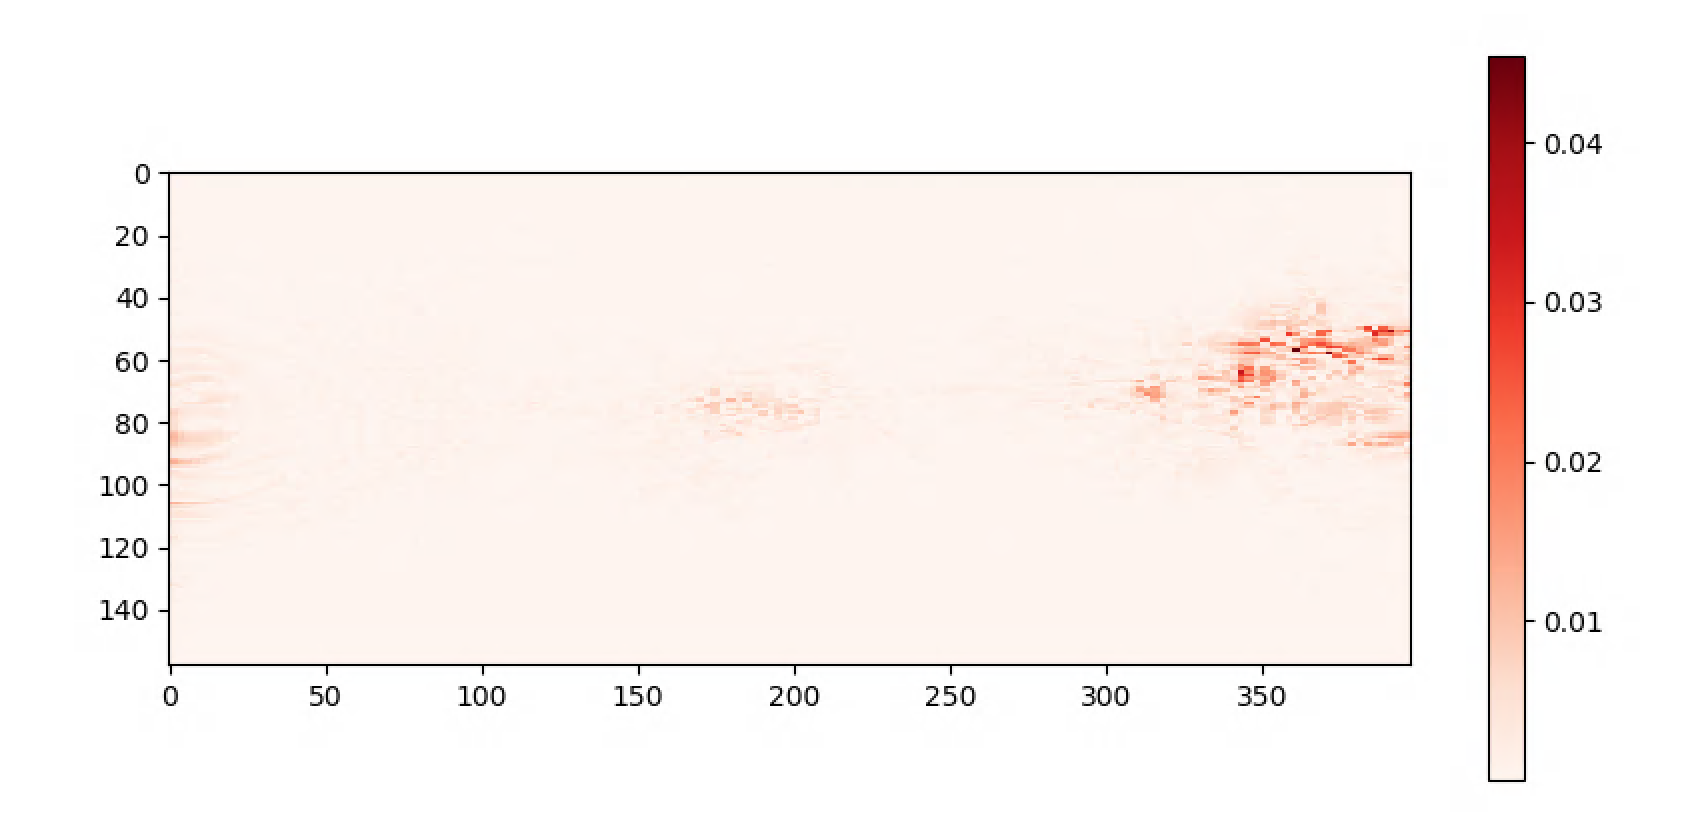
\includegraphics[width = 0.8\linewidth]{figures/350_12_error.png}
    \caption{Plot showing learning error (Case: 350 ambient jet)}
    \label{amr_err}
\end{figure}

\paragraph{Trained on 314 ambient tested on 350 ambient}

\begin{figure}[h!]
    \centering
    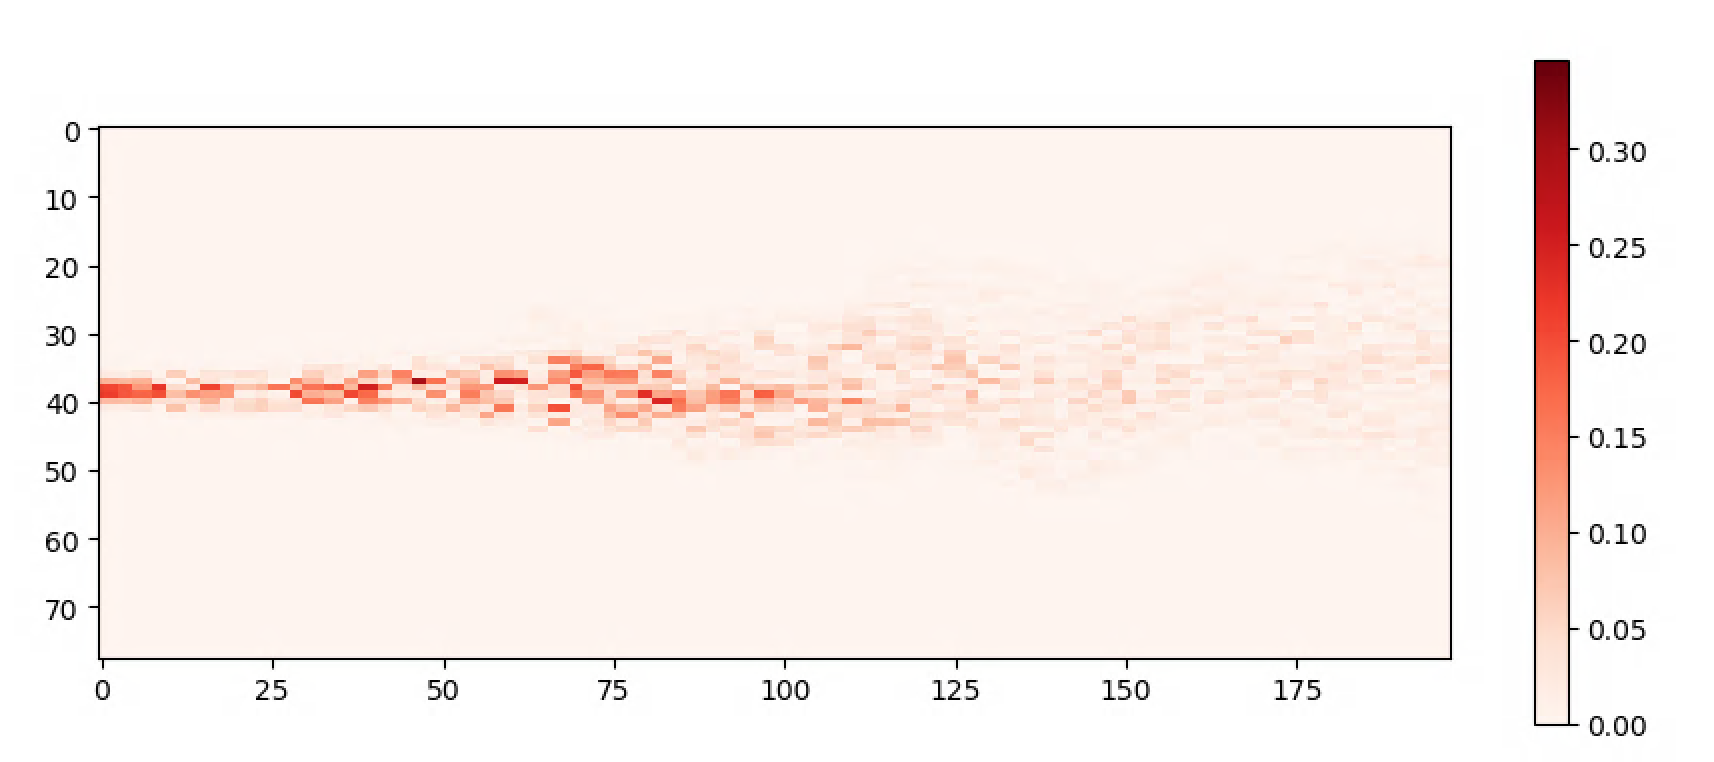
\includegraphics[width = 0.8\linewidth]{figures/314_350_01_actual.png}
    \caption{Plot showing actual error in $u$ computed from from level 1 run (Case: 350 ambient jet).}
    \label{amr_err}
\end{figure}

\begin{figure}[h!]
    \centering
    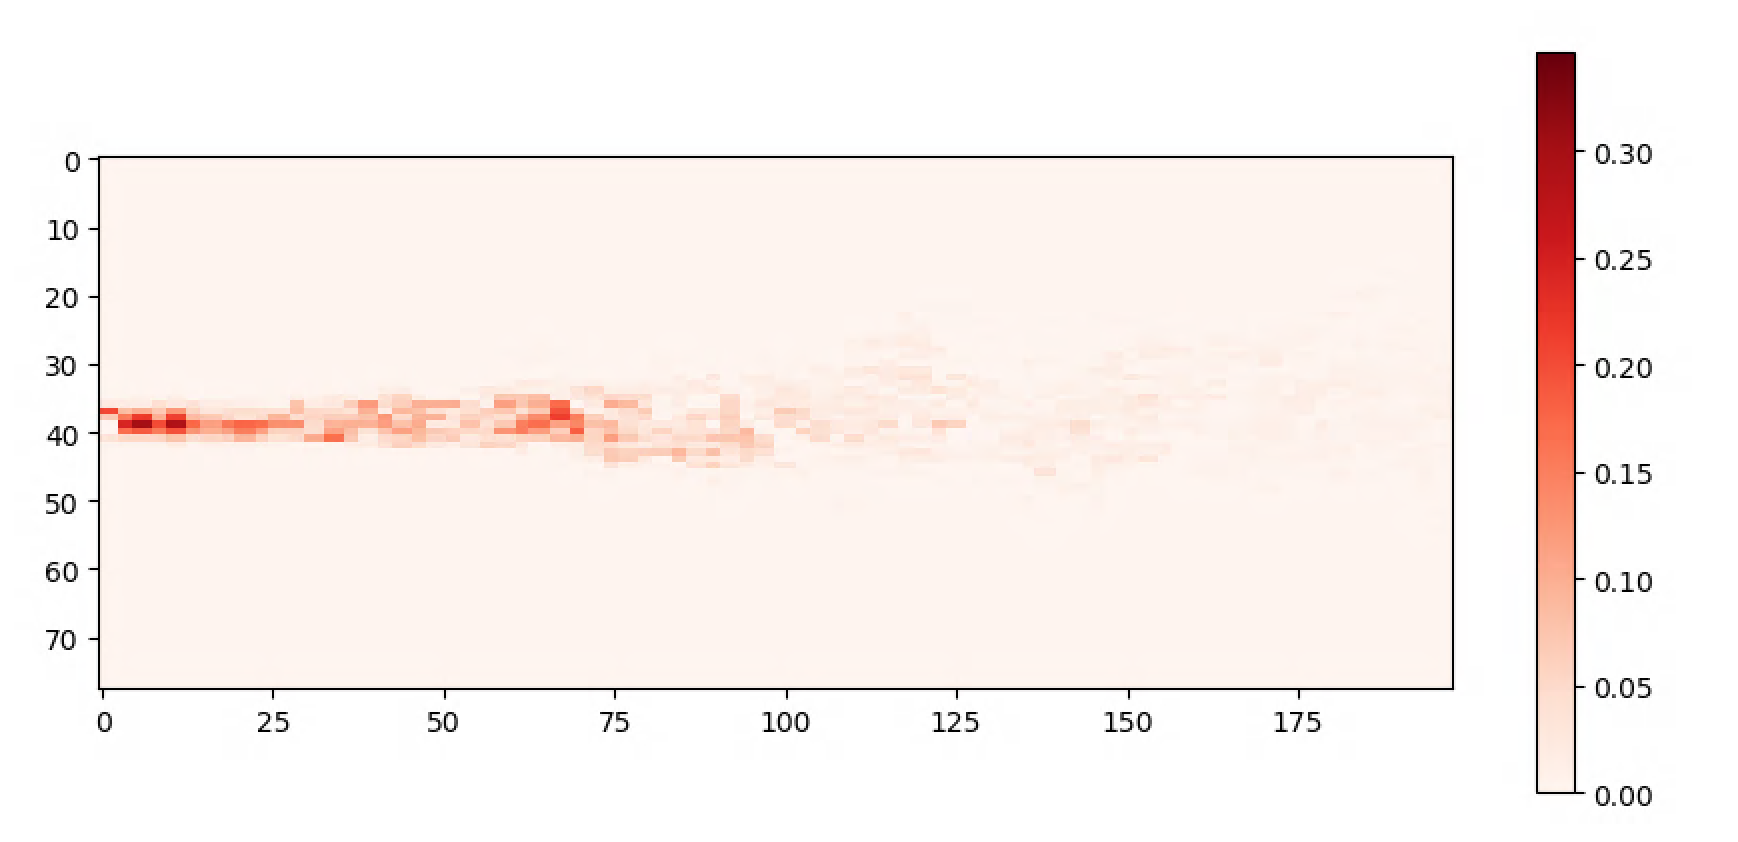
\includegraphics[width = 0.8\linewidth]{figures/314_350_01_pred.png}
    \caption{Plot showing predicted error in $u$ (Case: 350 ambient jet).}
    \label{amr_err}
\end{figure}

\begin{figure}[h!]
    \centering
    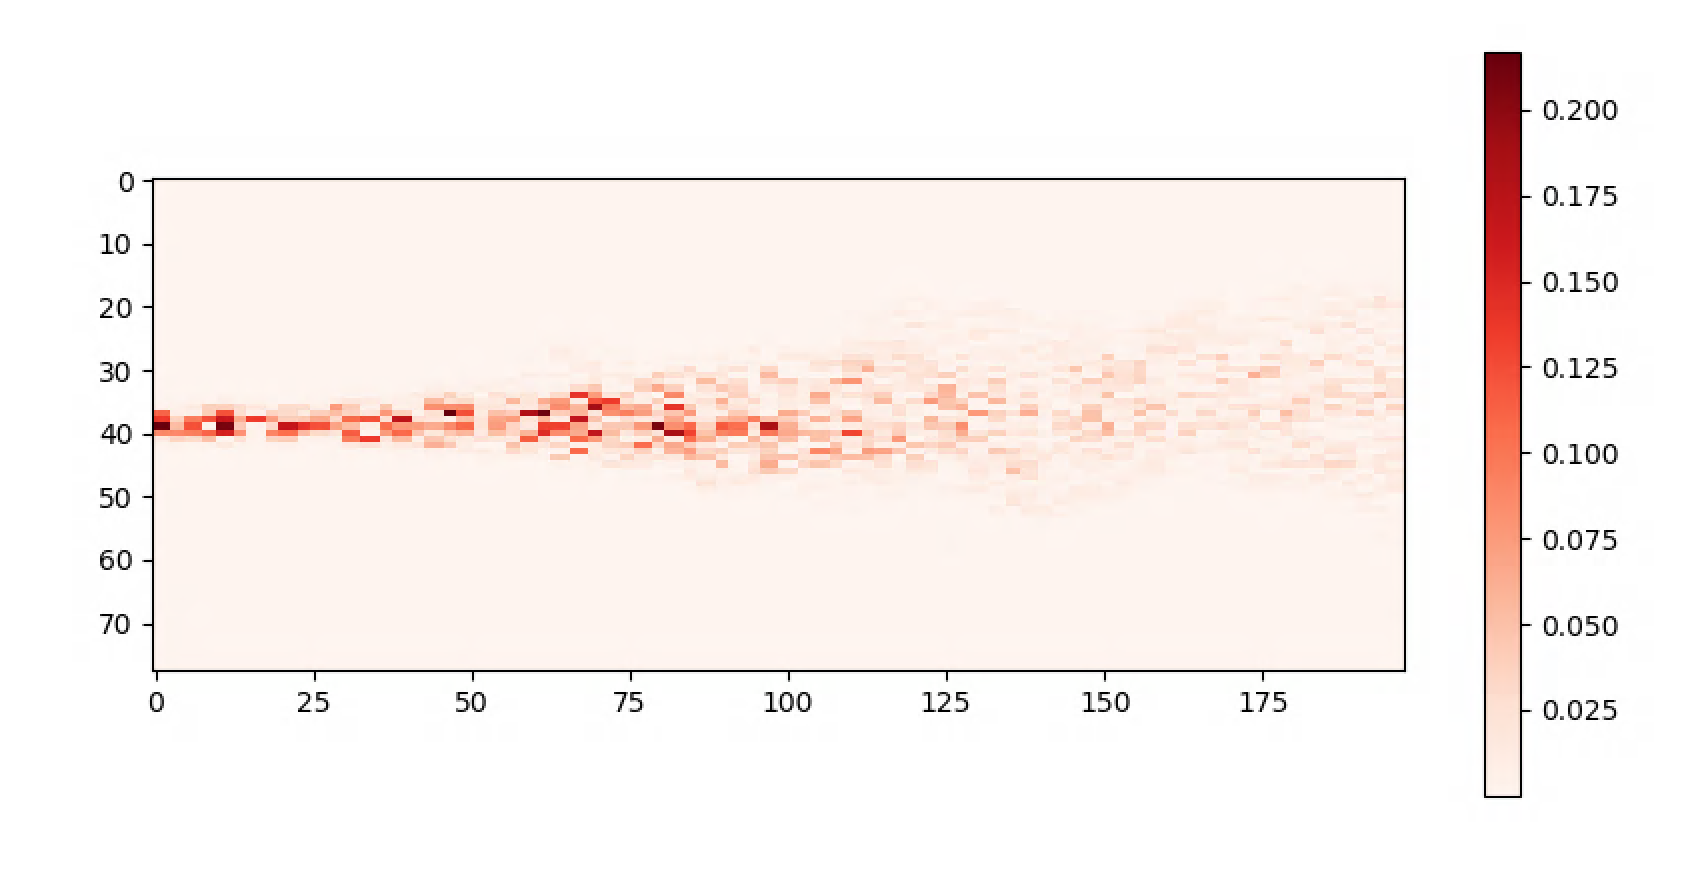
\includegraphics[width = 0.8\linewidth]{figures/314_350_01_error.png}
    \caption{Plot showing learning error (Case: 350 ambient jet)}
    \label{amr_err}
\end{figure}

\begin{figure}[h!]
    \centering
    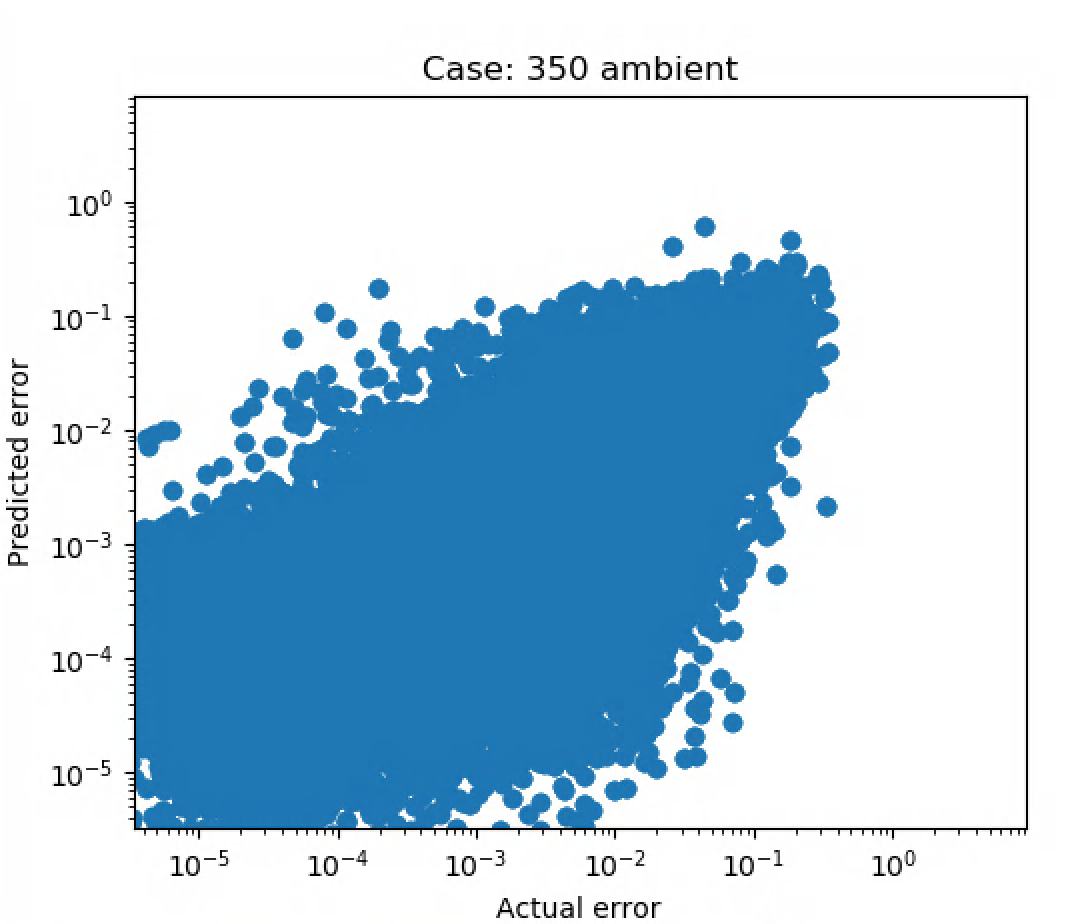
\includegraphics[width = 0.6\linewidth]{figures/314_350_01_error_scatter.png}
    \caption{Scatter plot showing actual vs predicted error (Case: 350 ambient jet)}
    \label{amr_err}
\end{figure}

\subsubsection{CNN}

\paragraph{314 ambient on base grid}

\begin{figure}[h!]
    \centering
    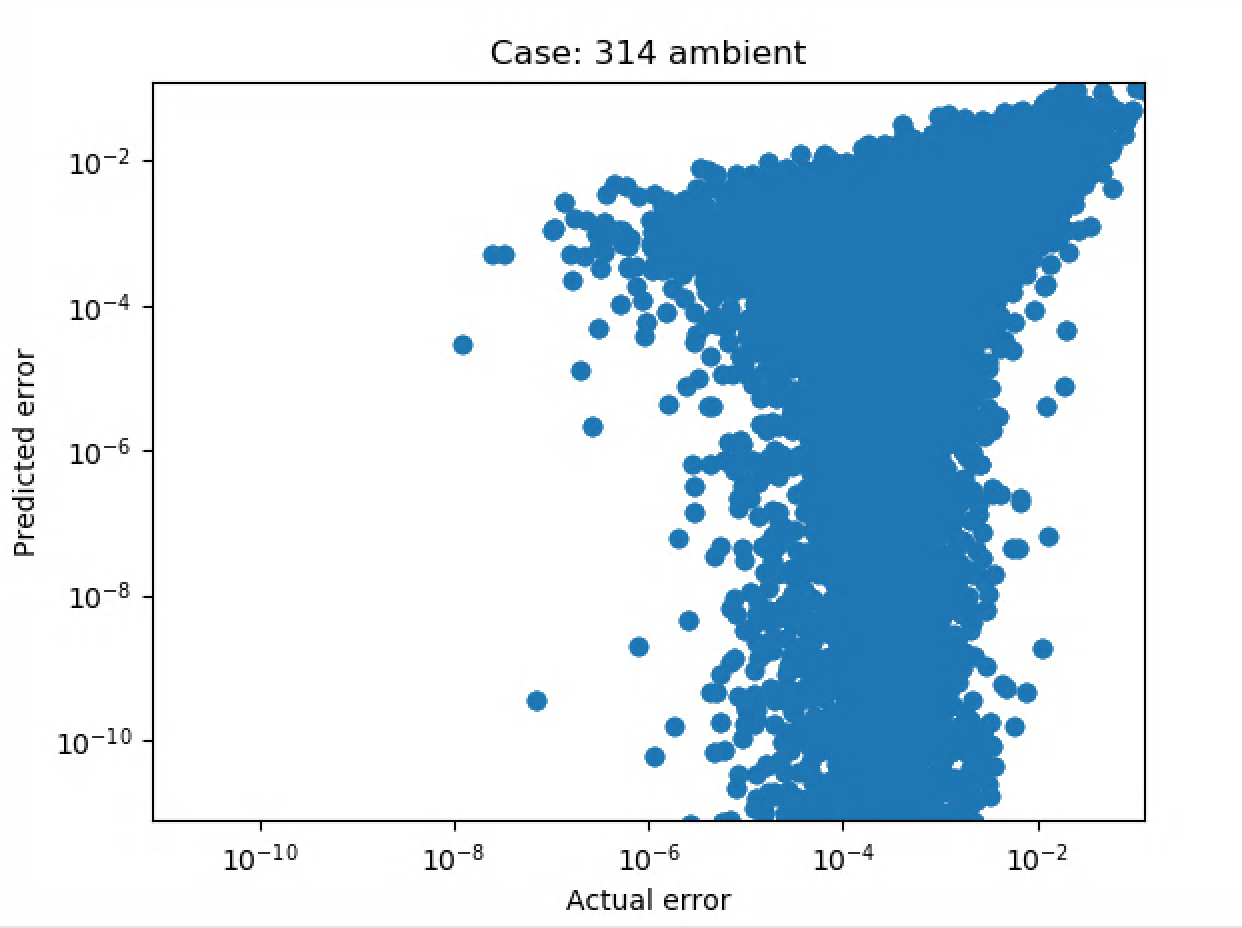
\includegraphics[width = 0.6\linewidth]{figures/314_01_cnn_error_scatter.png}
    \caption{Scatter plot showing actual vs predicted error (Case: 350 ambient jet)}
    \label{amr_err}
\end{figure}

\begin{figure}[h!]
    \centering
    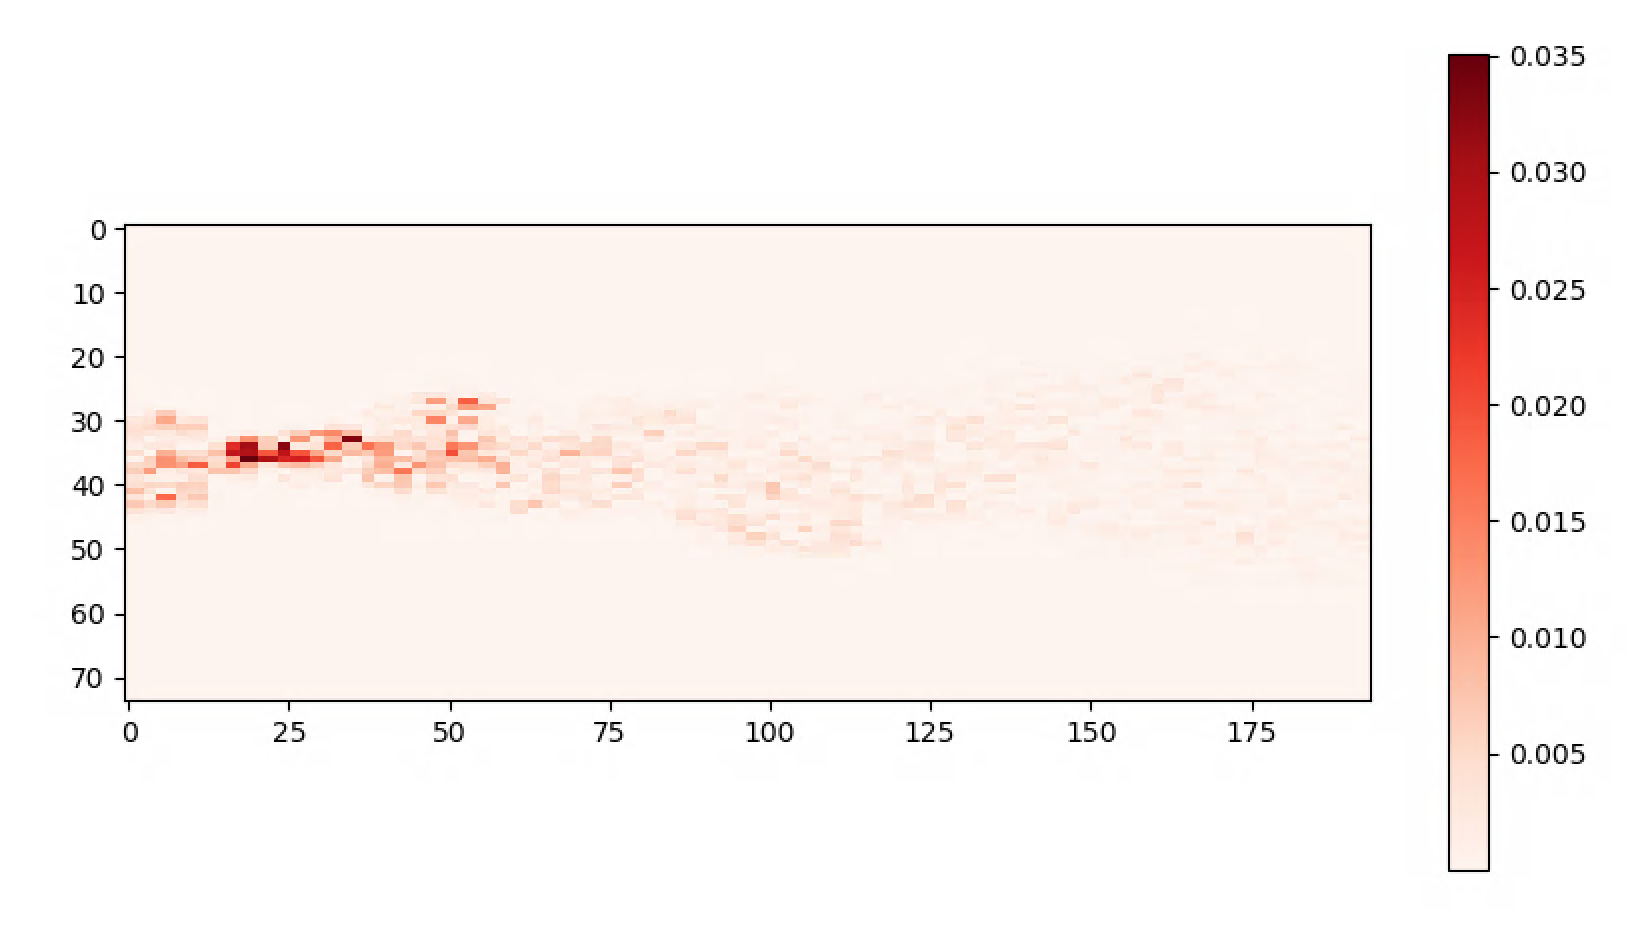
\includegraphics[width = 0.85\linewidth]{figures/314_01_cnn_actual.png}
    \caption{Plot showing actual error in $T$ computed from from level 1 run (Case: 314 ambient jet).}
    \label{amr_err}
\end{figure}

\begin{figure}[h!]
    \centering
    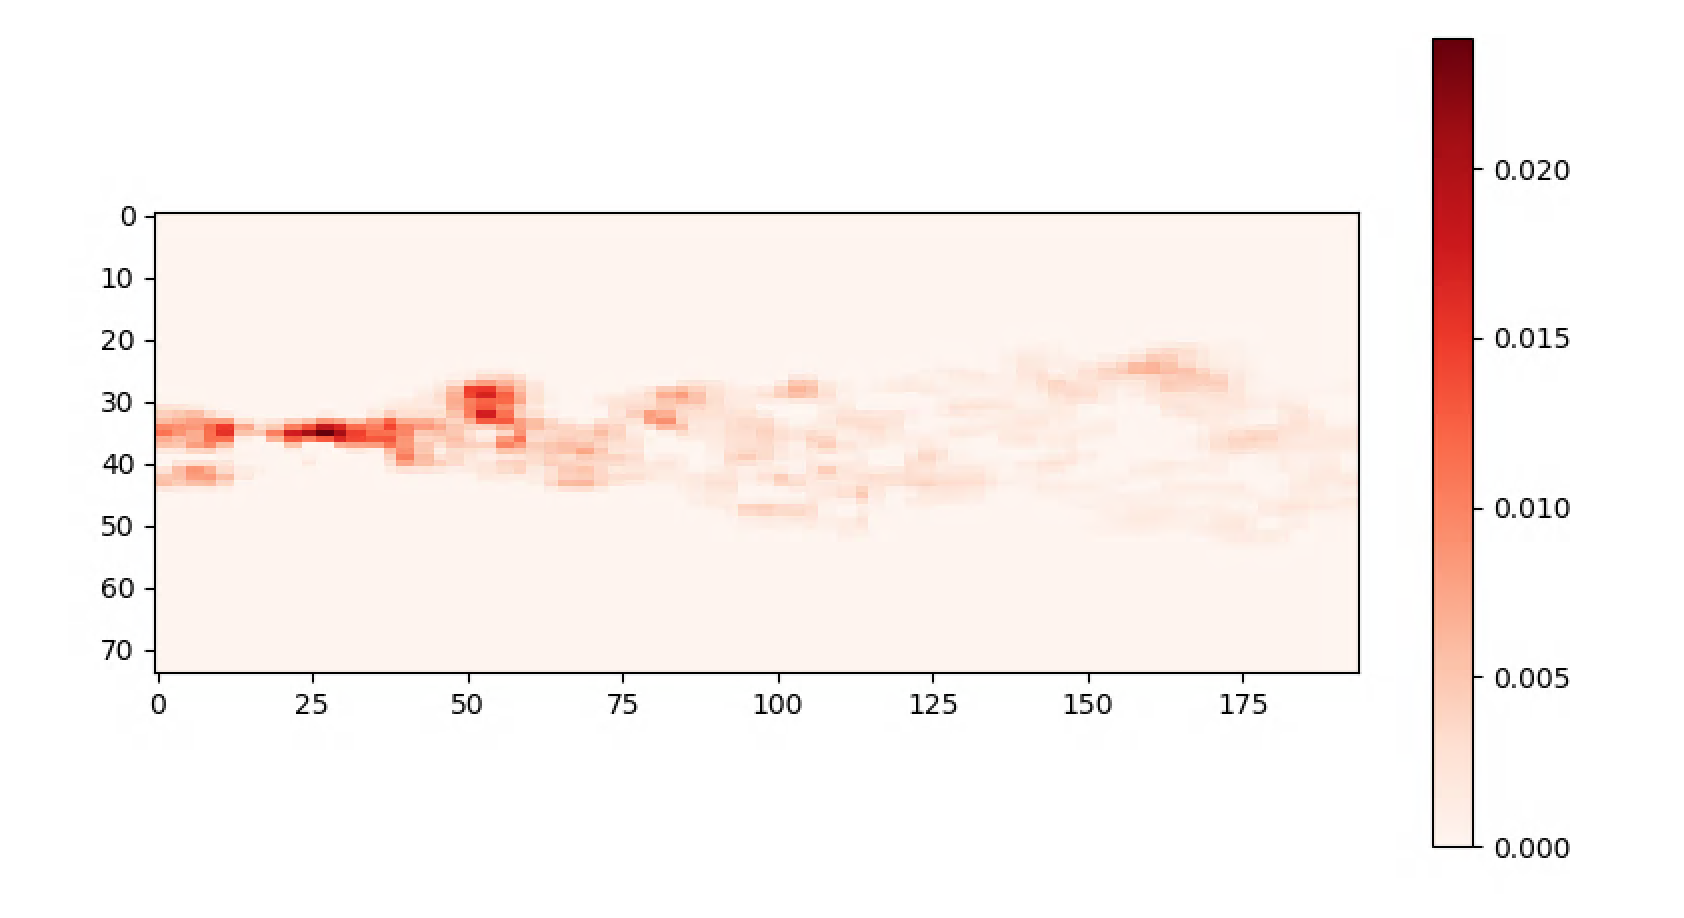
\includegraphics[width = 0.9\linewidth]{figures/314_01_cnn_pred.png}
    \caption{Plot showing predicted error in $T$.}
    \label{amr_err}
\end{figure}

\begin{figure}[h!]
    \centering
    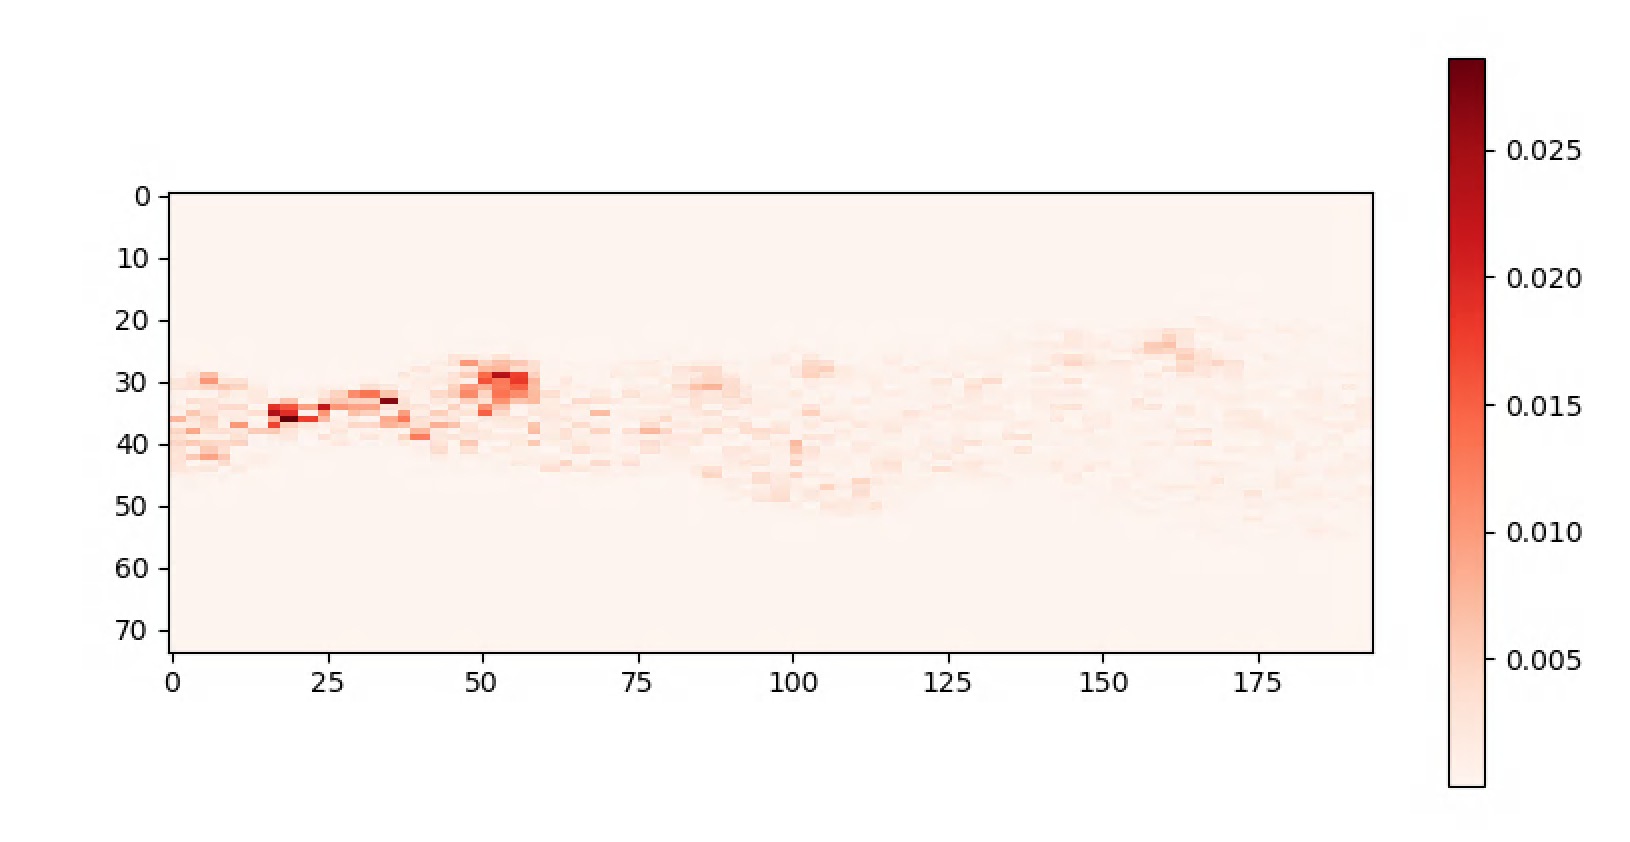
\includegraphics[width = 0.9\linewidth]{figures/314_01_cnn_error.png}
    \caption{Plot showing learning error (Case: 314 ambient jet)}
    \label{amr_err}
\end{figure}

\paragraph{314 ambient on base grid using gradients}

\begin{figure}[h!]
    \centering
    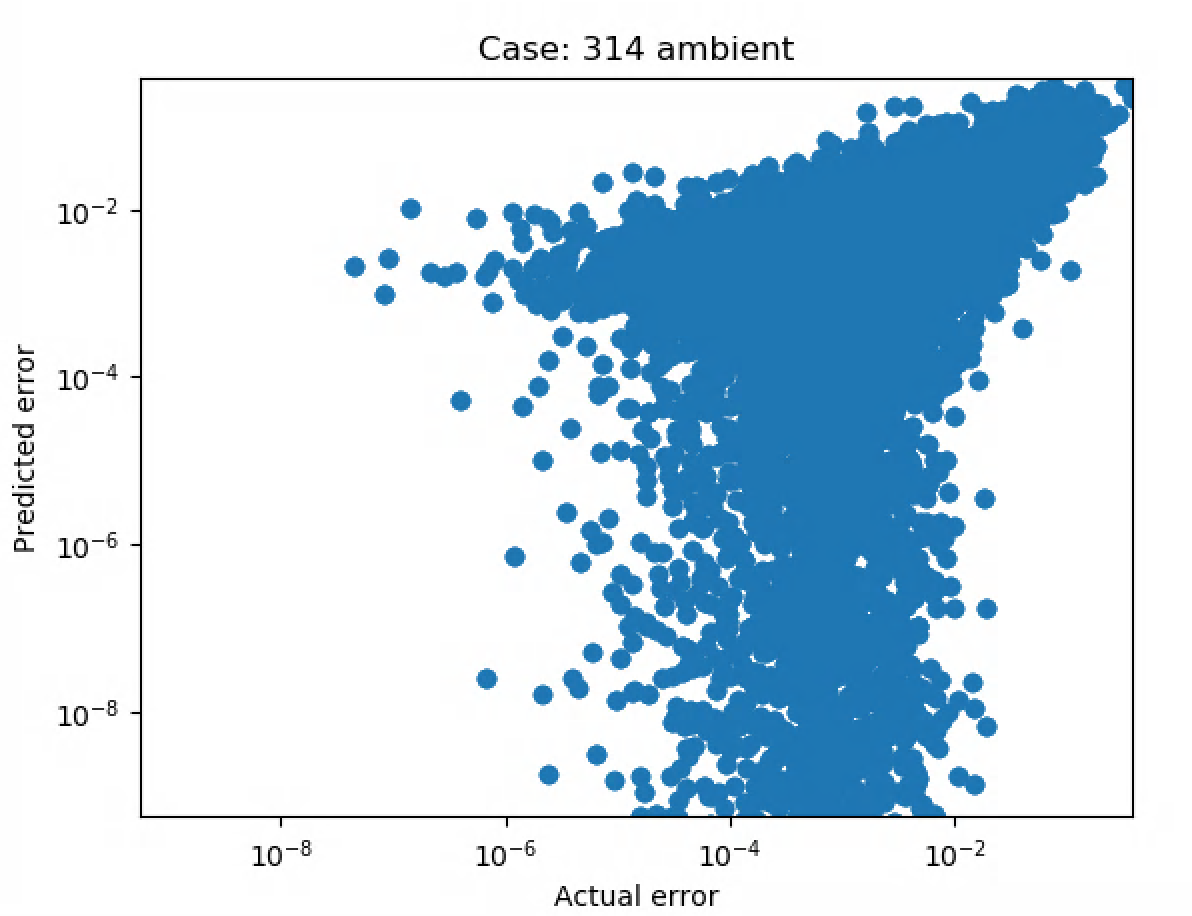
\includegraphics[width=0.6\linewidth]{figures/314_01_cnn_grad_error_scatter.png}
    \caption{Scatter plot showing actual vs predicted error (Case: 350 ambient jet)}
    \label{amr_err}
\end{figure}

\begin{figure}[h!]
    \centering
    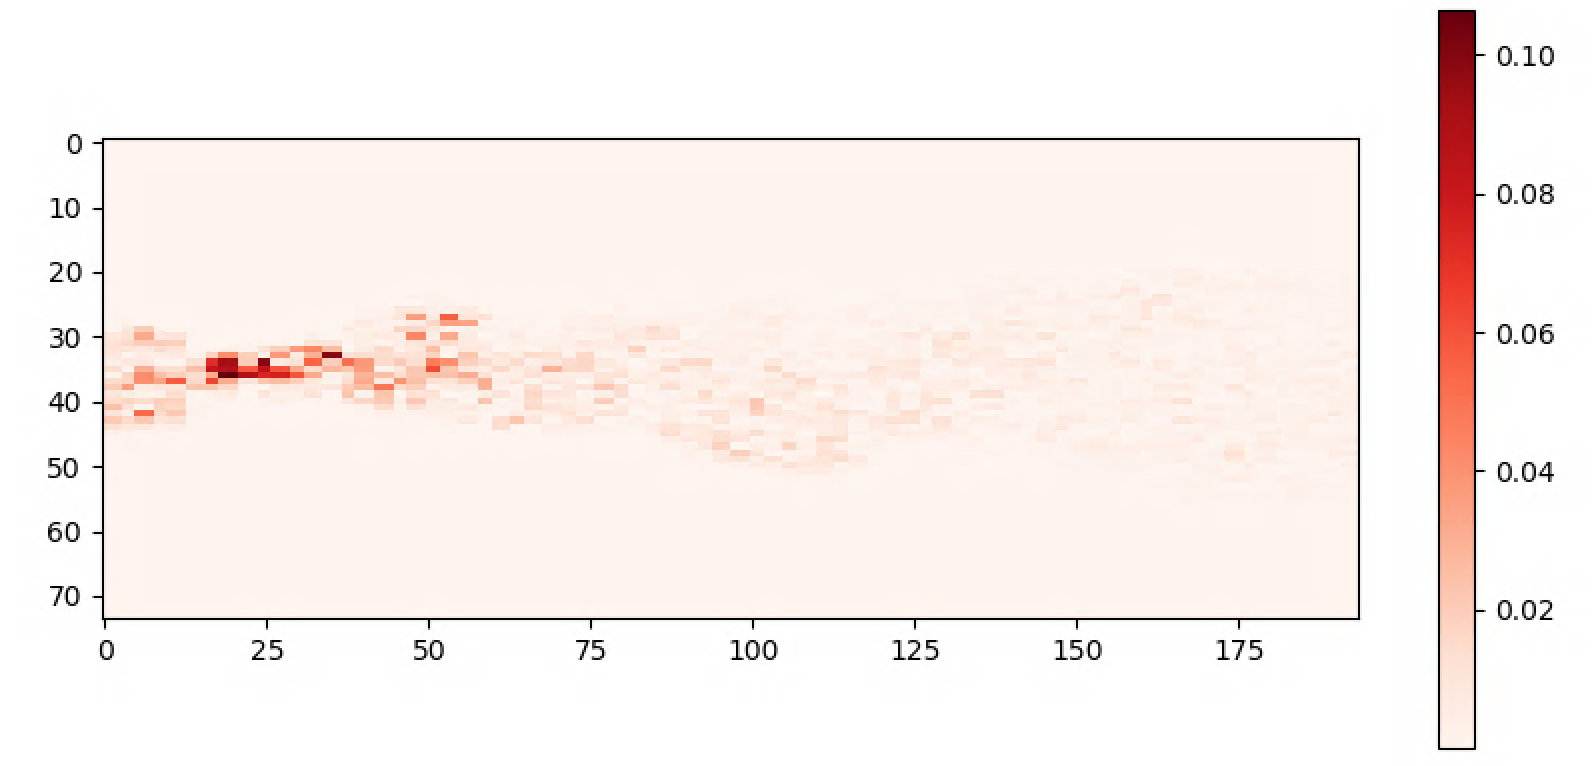
\includegraphics[width =0.85\linewidth]{figures/314_01_cnn_grad_actual.png}
    \caption{Plot showing actual error in $T$ computed from from level 1 run (Case: 314 ambient jet).}
    \label{amr_err}
\end{figure}

\begin{figure}[h!]
    \centering
    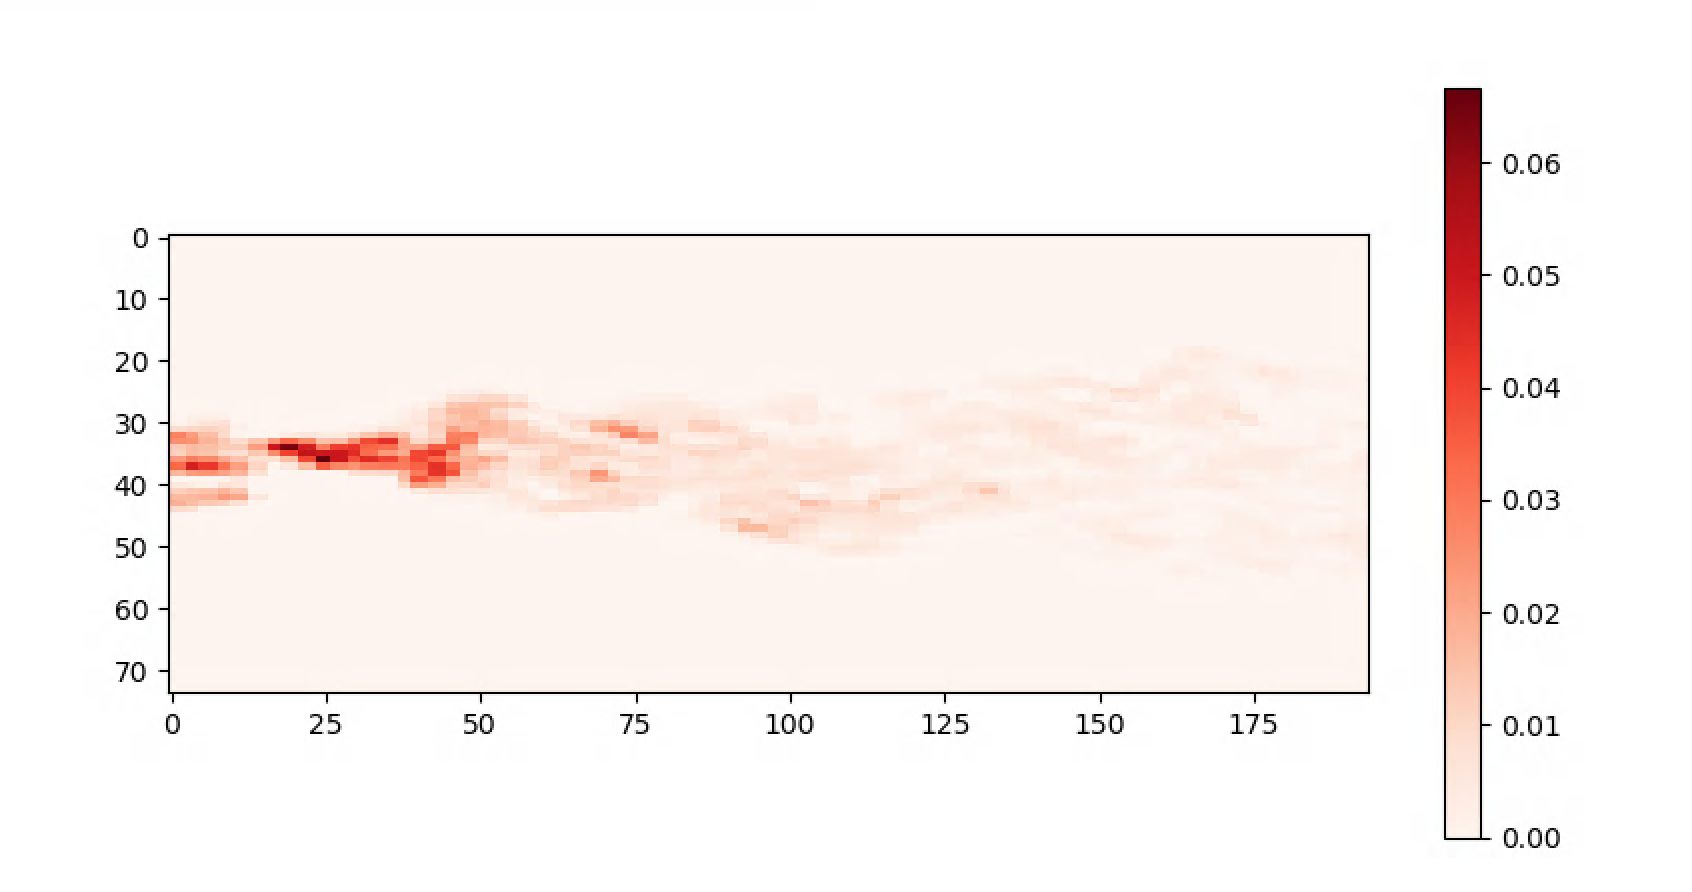
\includegraphics[width = 0.9\linewidth]{figures/314_01_cnn_grad_pred.png}
    \caption{Plot showing predicted error in $T$.}
    \label{amr_err}
\end{figure}

\begin{figure}[h!]
    \centering
    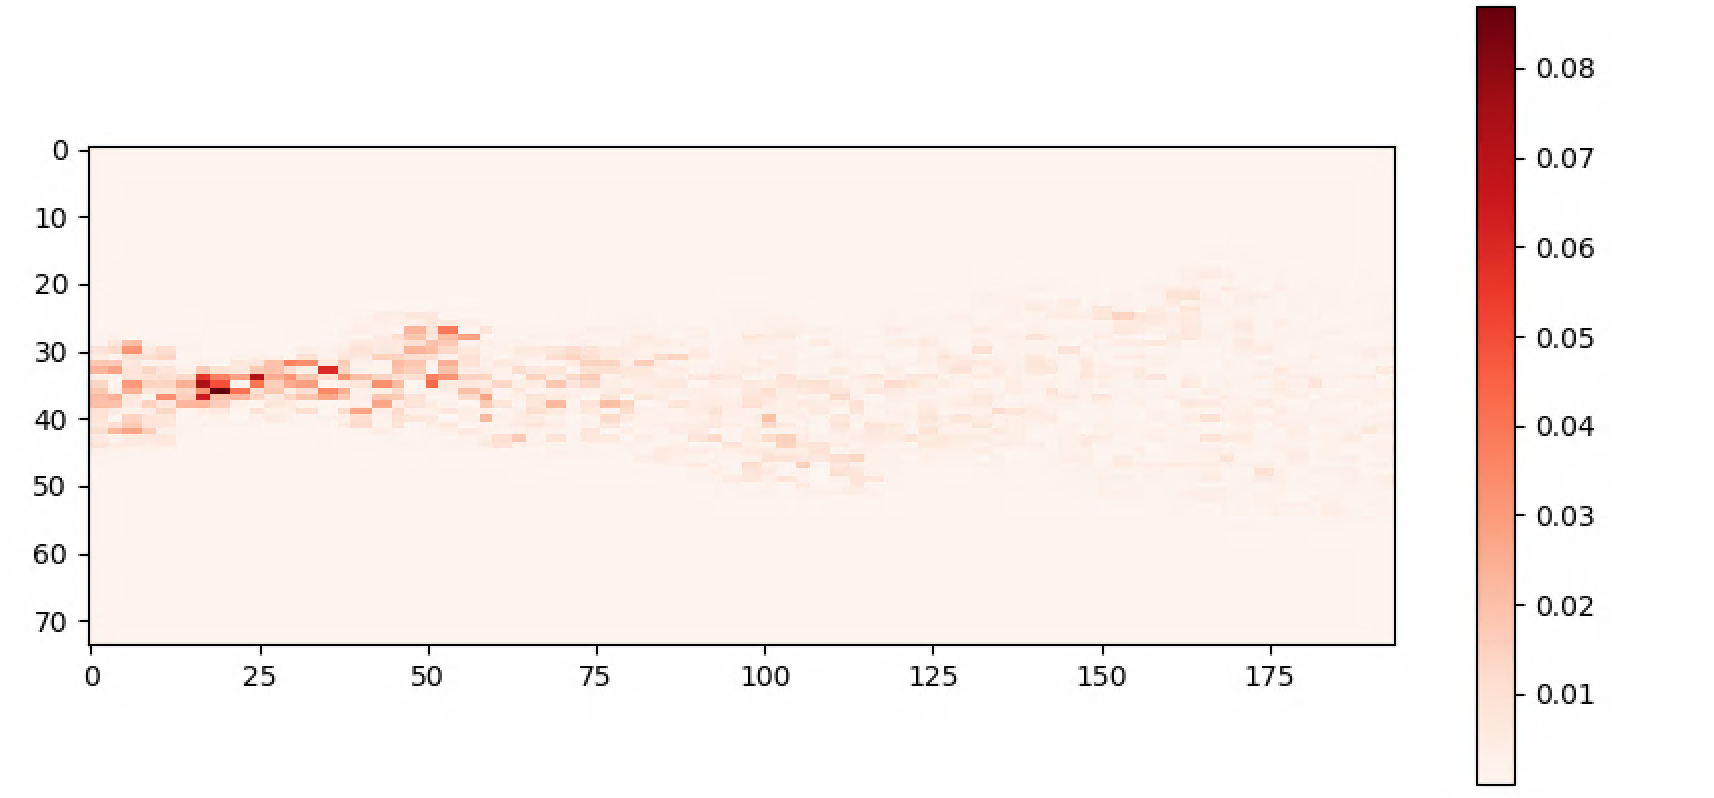
\includegraphics[width = 0.9\linewidth]{figures/314_01_cnn_grad_error.png}
    \caption{Plot showing learning error (Case: 314 ambient jet)}
    \label{amr_err}
\end{figure}

paragraph{Trained on 314 ambient on base grid using gradients, tested on 350 ambient}

\begin{figure}[h!]
    \centering
    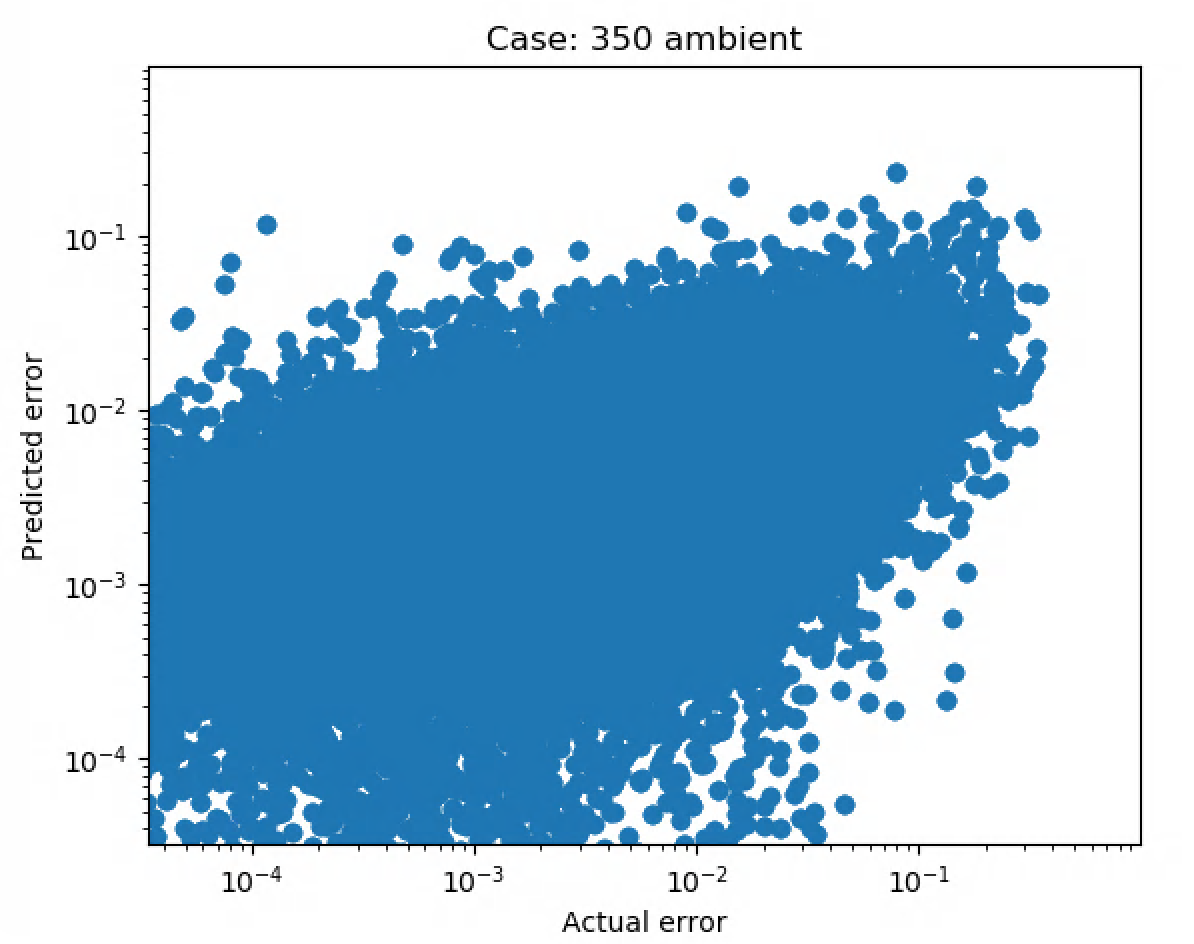
\includegraphics[width=0.6\linewidth]{figures/314_350_01_cnn_grad_error_scatter.png}
    \caption{Scatter plot showing actual vs predicted error (Case: 350 ambient jet)}
    \label{amr_err}
\end{figure}

\begin{figure}[h!]
    \centering
    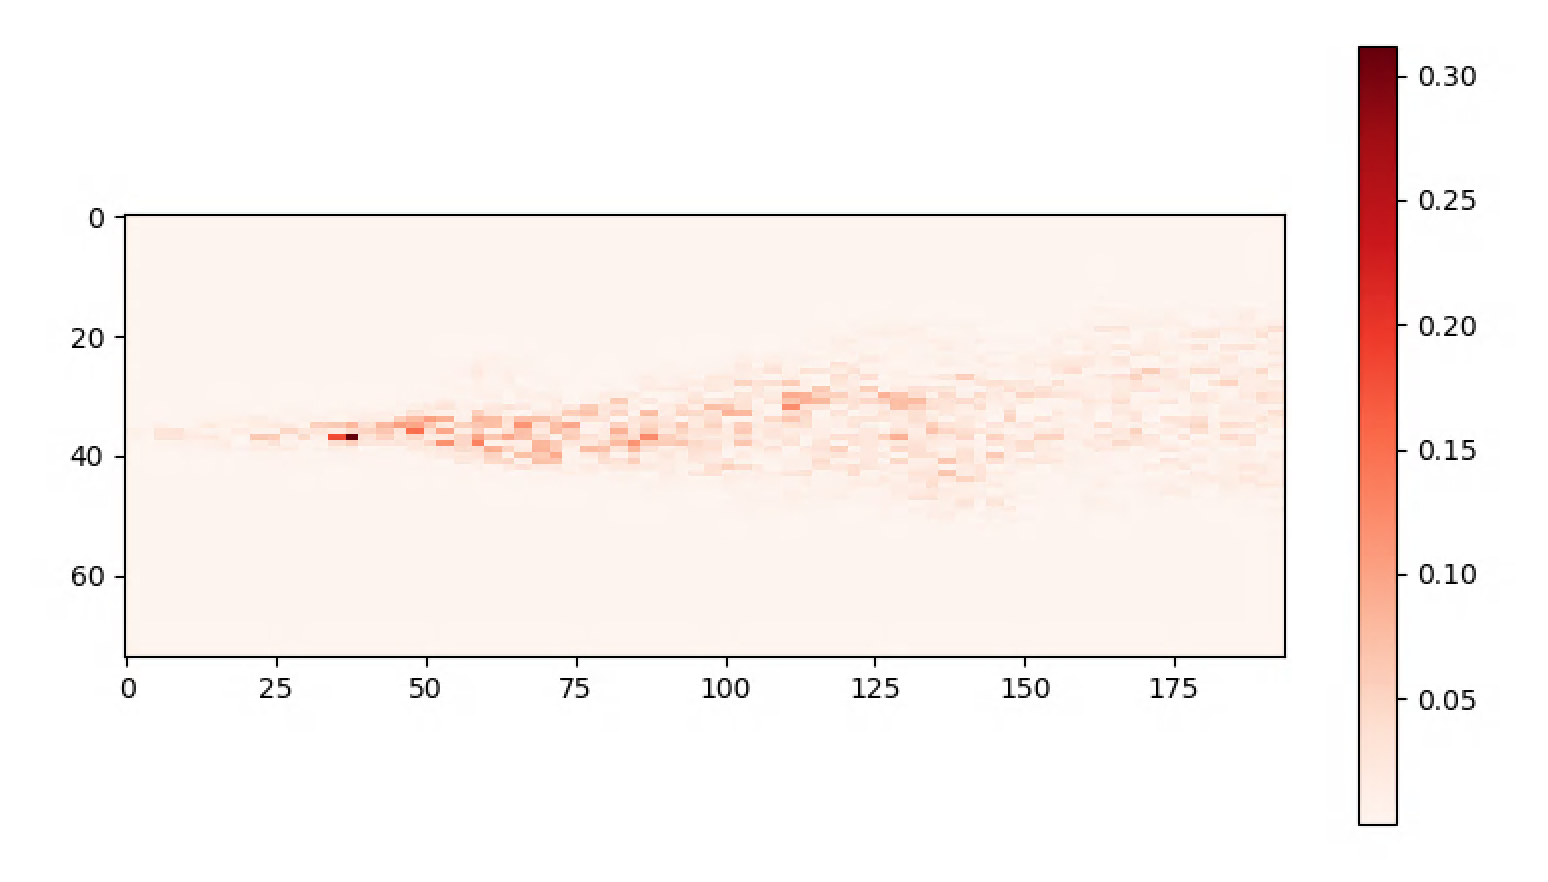
\includegraphics[width =0.85\linewidth]{figures/314_350_01_cnn_grad_actual.png}
    \caption{Plot showing actual error in $T$ computed from from level 1 run (Case: 350 ambient jet).}
    \label{amr_err}
\end{figure}

\begin{figure}[h!]
    \centering
    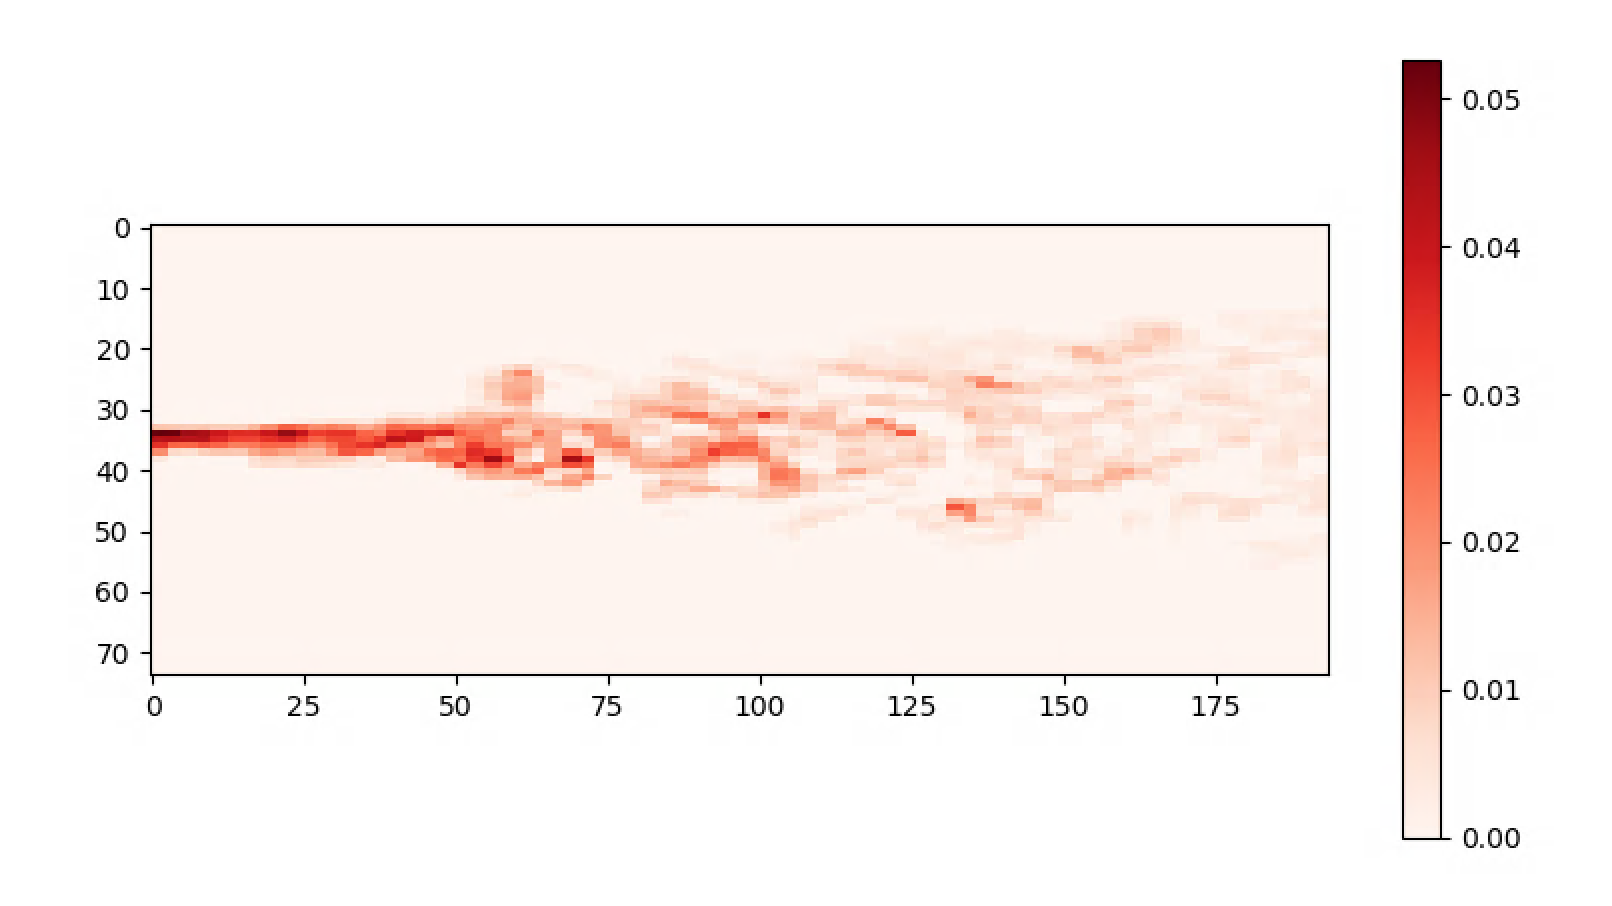
\includegraphics[width = 0.9\linewidth]{figures/314_350_01_cnn_grad_pred.png}
    \caption{Plot showing predicted error in $T$.}
    \label{amr_err}
\end{figure}

\begin{figure}[h!]
    \centering
    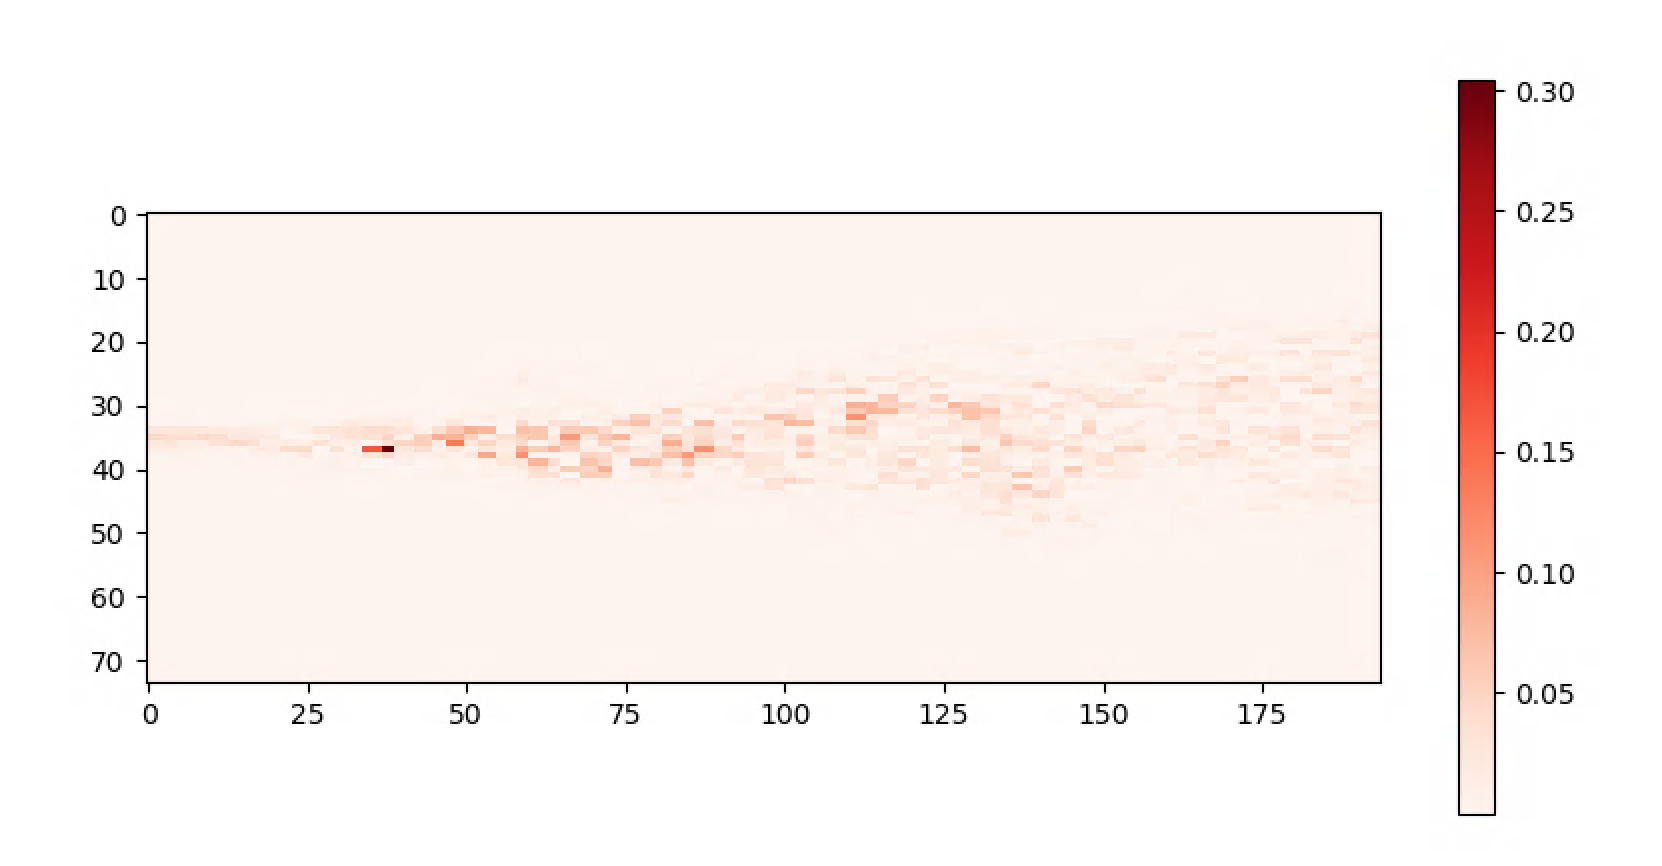
\includegraphics[width = 0.9\linewidth]{figures/314_350_01_cnn_grad_error.png}
    \caption{Plot showing learning error (Case: 314 ambient jet)}
    \label{amr_err}
\end{figure}

paragraph{Trained on 314 ambient on base grid, tested on 350 ambient}

\begin{figure}[h!]
    \centering
    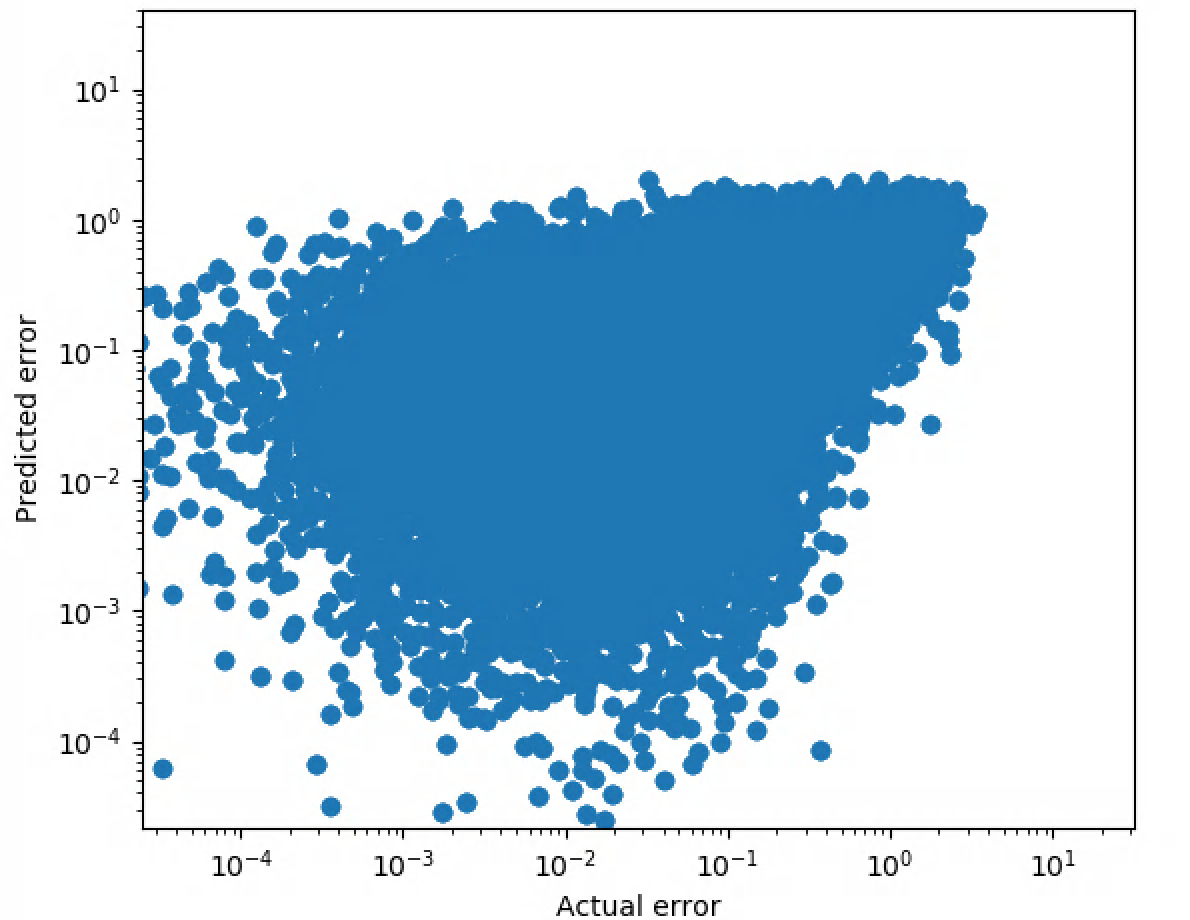
\includegraphics[width=0.6\linewidth]{figures/314_350_cnn_error_scatter.png}
    \caption{Scatter plot showing actual vs predicted error (Case: 350 ambient jet)}
    \label{amr_err}
\end{figure}

\begin{figure}[h!]
    \centering
    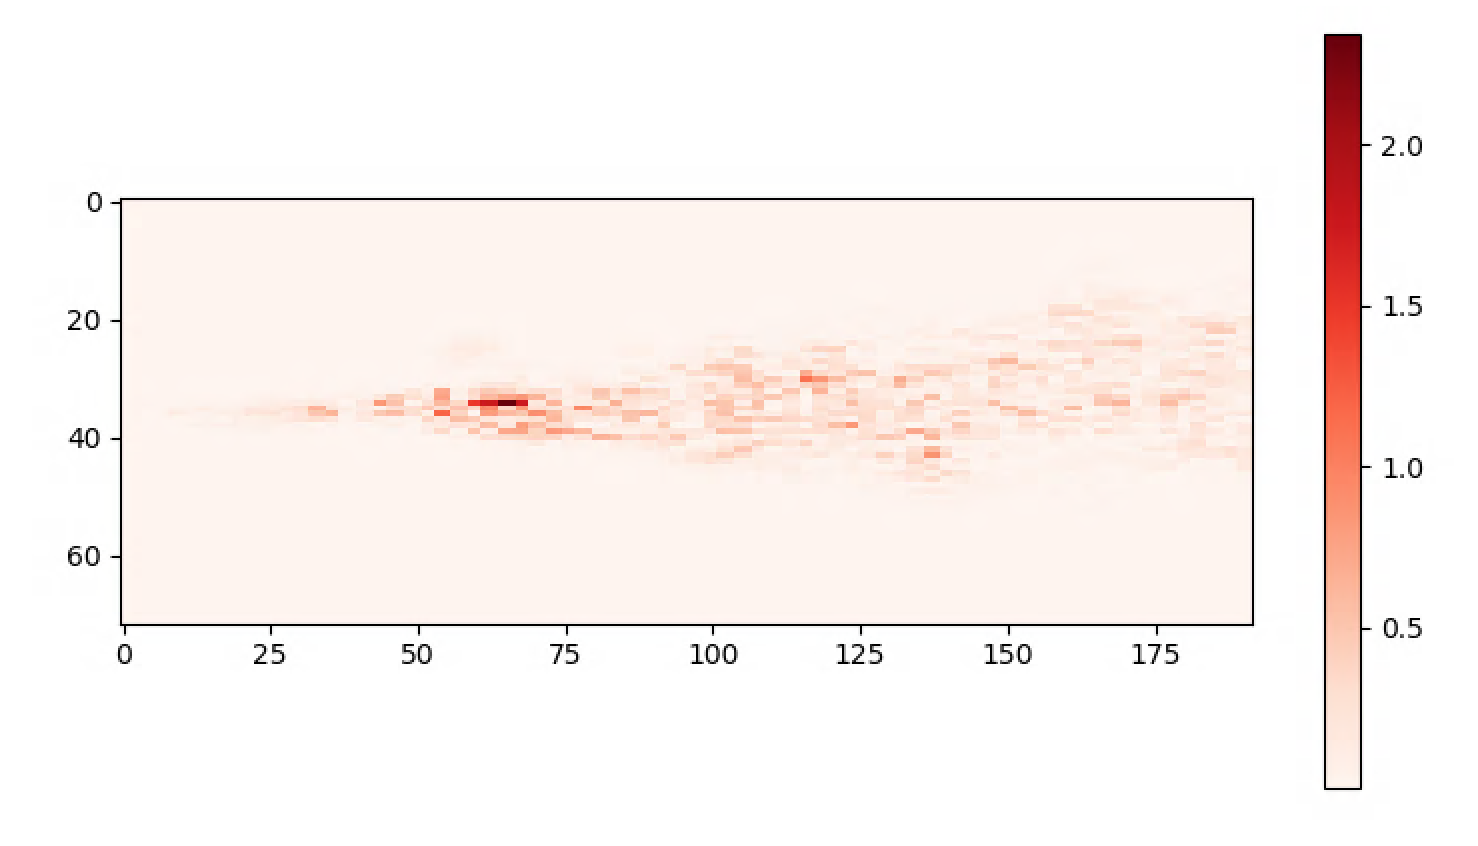
\includegraphics[width =0.85\linewidth]{figures/314_350_cnn_actual.png}
    \caption{Plot showing actual error in $u$ computed from from level 1 run (Case: 350 ambient jet).}
    \label{amr_err}
\end{figure}

\begin{figure}[h!]
    \centering
    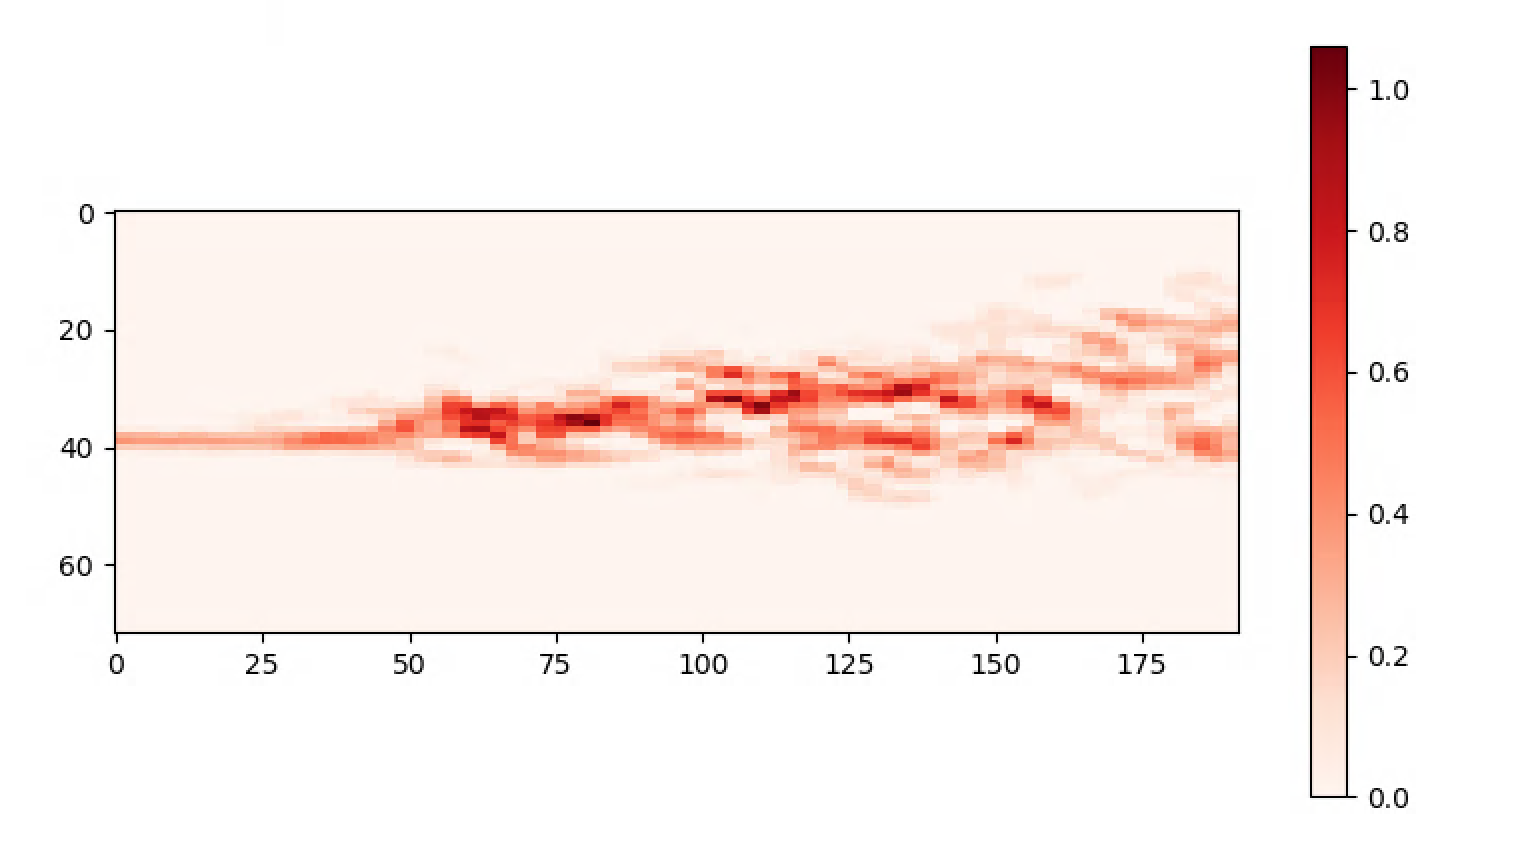
\includegraphics[width = 0.85\linewidth]{figures/314_350_cnn_pred.png}
    \caption{Plot showing predicted error in $u$.}
    \label{amr_err}
\end{figure}

\begin{figure}[h!]
    \centering
    \includegraphics[width = 0.9\linewidth]{figures/314_350_cnn_error.png}
    \caption{Plot showing learning error (Case: 314 ambient jet)}
    \label{amr_err}
\end{figure}

paragraph{Trained on 314 ambient on base grid, tested on 350 ambient (using slices)}

\begin{figure}[h!]
    \centering
    \includegraphics[width =0.85\linewidth]{figures/314_350_slices_actual.png}
    \caption{Plot showing actual error in $u$ computed from from level 1 run (Case: 350 ambient jet).}
    \label{amr_err}
\end{figure}

\begin{figure}[h!]
    \centering
    \includegraphics[width = 0.85\linewidth]{figures/314_350_slices_pred.png}
    \caption{Plot showing predicted error in $u$.}
    \label{amr_err}
\end{figure}

\begin{figure}[h!]
    \centering
    \includegraphics[width = 0.9\linewidth]{figures/314_350_slices_error.png}
    \caption{Plot showing learning error (Case: 314 ambient jet)}
    \label{amr_err}
\end{figure}

paragraph{Trained on 314 ambient on base + level 1 grid, tested on 350 ambient level 1 (fcnn)}

\begin{figure}[h!]
    \centering
    \includegraphics[width = 0.85\linewidth]{figures/314_01_12_350_12_error_scatter.png}
    \caption{Plot showing predicted error in $u$.}
    \label{amr_err}
\end{figure}


\begin{figure}[h!]
    \centering
    \includegraphics[width =0.85\linewidth]{figures/314_01_12_350_12_actual.png}
    \caption{Plot showing actual error in $u$ computed from from level 1 run (Case: 350 ambient jet).}
    \label{amr_err}
\end{figure}

\begin{figure}[h!]
    \centering
    \includegraphics[width = 0.9\linewidth]{figures/314_01_12_350_12_pred.png}
    \caption{Plot showing learning error (Case: 350 ambient jet)}
    \label{amr_err}
\end{figure}

\begin{figure}[h!]
    \centering
    \includegraphics[width = 0.9\linewidth]{figures/314_01_12_350_12_error.png}
    \caption{Plot showing learning error (Case: 350 ambient jet)}
    \label{amr_err}
\end{figure}



\section{Normalization and Hyperparameter optimization studies based on Temperature error prediction}

\begin{table}
\centering
\begin{tabular}{llllll}
 &Input  &Label normalized   &Normalized wrt to original data &mse &mse(new)   \\
 &Raw ($3 \times 3 \times 3$)  &no  &no  &15  &154 \\
 &Grad ($3 \times 3 \times 3$) &no  &no  &12  &14\\
 &Grad ($1 \times 1 \times 1$) &no  &no  &97  &1682\\
 &Raw ($3 \times 3 \times 3$)  &no  &yes &12  &1176 \\
 &Grad ($3 \times 3 \times 3$) &no  &yes &12  &65\\
 &Raw ($3 \times 3 \times 3$)  &yes &no &$0.94 \times (5.4)^2$  &$0.53 \times (5.4)^2$ \\
 &Grad ($3 \times 3 \times 3$) &yes  &no &$0.97 \times (5.3)^2$  &$0.52 \times (5.3)^2$ \\
\end{tabular}
\end{table}

\begin{table}
\centering
\begin{tabular}{llll}
 &Parameter  &Range   &Optimal    \\
 &Learning rate  &$[0.0001,0.001]$  &$0.0004$  \\
 &Dropout rate   &$[0,0.4]$  &$0.36$  \\
 &Batch size &${16,32,64,128,256}$  &128  \\
 &Hidden units & ${8,16,32,64,128}$  &64 \\
\end{tabular}
\end{table}

\begin{table}
\centering
\begin{tabular}{llll}
 &Parameter  &Range   &Optimal    \\
 &Learning rate  &$[0.0001,0.001]$  &$0.00013$  \\
 &Dropout rate   &$[0,0.4]$  &$0.11$  \\
 &Batch size &${16,32,64, 128,256}$  &32  \\
 &Number of filters & ${4,8,16,32,64}$  &4 \\
 &Hidden units & ${4,8,16,32}$  &8 \\
\end{tabular}
\end{table}


\end{document}
